Events in which $Z$ bosons are produced in association with jets account for a large fraction of the high-$\met$ all-hadronic events at the LHC. Not surprisingly, these events are a major background to new physics that may manifest signals in the hadronic channel. Since the jet multiplicity beyond 4 jets, as well as the relationships between the directions of jets, are not simulated accurately, it is generally advisable to employ data-driven methods for $\zinv$ background estimation, especially when the signal region is populated by events with several jets. Typically, data-driven approaches make use of similarities between the kinematics of $\zinv$ events and $Z\rightarrow X\bar{X}$ events, where $X$ is one of the other $Z$ boson decay products, or of the similarities between events with $Z$ bosons and events with photons. The former approach is adopted in the following.


\subsection{The relationship between $\zinv$ and $\zll$}
The kinematics of $Z$ bosons are independent of the decay mode of the $Z$ boson, as is the case for any particle that can undergo a variety of decays. The decay modes and branching fractions $\mathcal{B}$ for the $Z$ boson are listed in Table \ref{tab:zdecay}. 

\begin{table}[h]
\vspace{0.5cm}
\centering
\begin{tabular}{l|rl}
\hline
decay mode & \multicolumn{2}{c}{$\mathcal{B}$(\%)}\\
\hline
e$^+$e$^-$ & $3.363$&\hspace{-3mm}$\pm \hspace{1mm}0.004$\\
$\mu^+\mu^-$ & $3.366$&\hspace{-3mm}$\pm \hspace{1mm}0.007$\\
$\tau^+\tau^-$ & $3.370$&\hspace{-3mm}$\pm \hspace{1mm}0.008$\\
$\nu\bar{\nu}$ & $20.00$&\hspace{-3mm}$\pm \hspace{1mm}0.06$\\
q$\bar{\text{q}}$ & $69.91$&\hspace{-3mm}$\pm \hspace{1mm}0.06$\\
\hline
\end{tabular}
\caption{The measured decay modes of the $Z$ boson, as reported in \cite{Agashe:2014kda}.}
\label{tab:zdecay}
\end{table}

Events featuring the $\zinv$ decay mode are largely indistinguishable from other events with $\met$ and no leptons, and therefore obtaining a reasonably pure data sample of $\zinv$ events is not feasible. However, events with $\zll$ decays can be selected with high purity by requiring two opposite-sign, same-flavor, well-isolated leptons, whose invariant mass falls within a range similar to $|m_{ll}-m_\text{Z}|<20$ GeV. For events in such a sample, the $Z$ boson can be reconstructed by summing the four-vectors of the two leptons, and if the $Z$ is removed from the event, a proxy sample for real $\zinv$ events is obtained. The process of removing the tagged $Z$ boson is referred to as event cleaning. 

The resulting ``cleaned'' event sample is expected to exhibit {\it all} the characteristics of the real $\zinv$ events, barring two exceptions: first, distributions of extensive properties derived from the $l\bar{l}$ sample will be too low by an overall normalization factor of $20/3.4\approx5.9$ because of the difference in branching fractions of the $\zinv$ and $\zll$ decay modes; and second, the shapes of distributions based on the $\zll$ sample will be altered because the acceptance, reconstruction efficiency, and isolation efficiency of the lepton selection. To correct for the first difference, $\zll$-derived distributions are scaled up by the normalization factor 5.9. To correct for the second difference, events in the $\zll$ sample are weighted by the inverse of the lepton efficiencies mentioned. The prediction for the $\zinv$ count $N_i$ in a given signal region $i$ is therefore given by
\begin{equation}
N_i = N_i(\zll)\cdot\frac{1}{\epsilon^{\text{Z}}_{\text{acc}}}\cdot\frac{1}{\epsilon^{\text{Z}}_{\text{rec}}}\cdot\frac{1}{\epsilon^{\text{Z}}_{\text{iso}}}\cdot\frac{\mathcal{B}(\zinv)}{\mathcal{B}(\zll)},
\label{eq:zinv}
\end{equation}
where $N_i(\zll)$ is the observed count in signal region $i$ from the cleaned dilepton sample, and the $\epsilon^{\text{Z}}$'s are the efficiencies of acceptance, reconstruction, and isolation.

\subsection{Procedure with 13 TeV data} 
A procedure was developed previously \cite{CMS:2016nhb} to estimate the $\zinv$ counts using events with two opposite-sign muons, using simulated events as well as real events collected in 2015. Muon events were chosen rather than electron events, since the muon efficiency is roughly 10\% larger than the electron efficiency, a choice that yields the larger of the two dilepton samples. However, the number of real events containing $\zmumu$ decays are limited because of the integrated luminosity recorded in 2015 is relatively small, and so an estimate of the $\zinv$ count could not be made in all signal regions. Thus, a data-simulation hybrid approach was taken, detailed in Ref. \cite{CMS:2016nhb}, in which simulated $\zinv$ events are reweighted based on the ratio of counts between data and simulation in bins of jet multiplicity and b-jet multiplicity, and are subsequently taken as the prediction. Systematic uncertainties, as well as the weights, are derived in control regions believed to be signal-poor; the systematic effects include those associated with the normalization uncertainty, shape uncertainties, and uncertainties associated with the reweighting. 

I developed the method to incorporate a data event sample with two opposite-sign electrons to complement, and further constrain, the $\zinv$ background prediction. On its own, the ee-based prediction is not expected to yield a better prediction, namely, a prediction with smaller uncertainties, than the $\mu\mu$-based prediction; however, given that electron and muon efficiencies are comparable within about 10\%, the combination of $\mu\mu$ and ee data should result in a reduction in control region statistical uncertainties by $\approx$ 30\%. 

Reconstructed electrons are selected with $\pt$ greater than 33 (36) GeV, a threshold chosen to ensure the double electron trigger,
\begin{itemize}
  \item \texttt{HLT\_DoubleEle33\_CaloIdL\_GsfTrkIdVL\_MW\_v},
\end{itemize}
has a nearly 100\% probability of selecting electrons passing the kinematic selection. Electrons are also required to be isolated.  An isolated electron has an isolation value less than 0.1,  where isolation is defined as the ratio of the $\pt$ sum of reconstructed particles within a $\Delta R$ cone around the lepton (excluding the lepton) to the $\pt$ of the lepton, where the cone size R varies with the the lepton $\pt$:
\begin{equation}
\text{isolation} = \sum_{i}(p_{T})_i \cdot \Theta[R^*-\Delta R_{i})]/(p_T)_{\text{lepton}},
\label{eq:isolation}
\end{equation}
\[
R^* = 
  \begin{cases} 
  0.2 & \text{: } \pt \leq 50 \text{ GeV} \\
  (10 \text{ GeV})/\pt & \text{: } 50 < \pt \leq 200 \text{ GeV} \\  
   0.05 & \text{: } \pt > 200 \text{ GeV}. \\
  \end{cases}
\]
\noindent 

An essential objective is finding a suitable parametrization of the efficiencies, $\epsilon^{\text{Z}}_{\text{acc}}$, $\epsilon^{\text{Z}}_{\text{rec}}$, and $\epsilon^{\text{Z}}_{\text{iso}}$, that will result in the shapes of distributions derived from the cleaned ee sample agreeing with those of the $\zinv$ events. Since it is not the $Z$ bosons themselves that are reconstructed, but their decay products, a good parametrization must incorporate information about the leptons, but characterize the $Z$ boson itself.  This approach is distinct from the approach taken in the $\mu\mu$ method where the efficiencies are parametrized in terms of properties of individual leptons, and the efficiencies for the two leptons in each event are multiplied to yield an event-level efficiency. The efficiency maps are now presented, based on the parametrization that was ultimately chosen. 

\subsubsection{Acceptance $\epsilon^{\text{Z}}_{\text{acc}}$}
The acceptance is defined as the fraction of $\zee$ events where both electrons satisfy the kinematic criteria
\begin{itemize}
\item $\pt>33$ GeV
\item $|\eta|<2.5$.
\item $|m_{ll}-m_{\text{Z}}|<20$ GeV
\end{itemize}
Since the $Z$ boson $\pt$ and $\eta$ are correlated with but not equal to the $\pt$ and $\eta$ of both electrons, these observables are a well-suited option for the acceptance parametrization. Figure \ref{fig:ZeeAcceptance} shows the acceptance as a function of the inferred $Z$ boson $\eta$ and $\pt$. 
\begin{figure}[tb!]
\centering
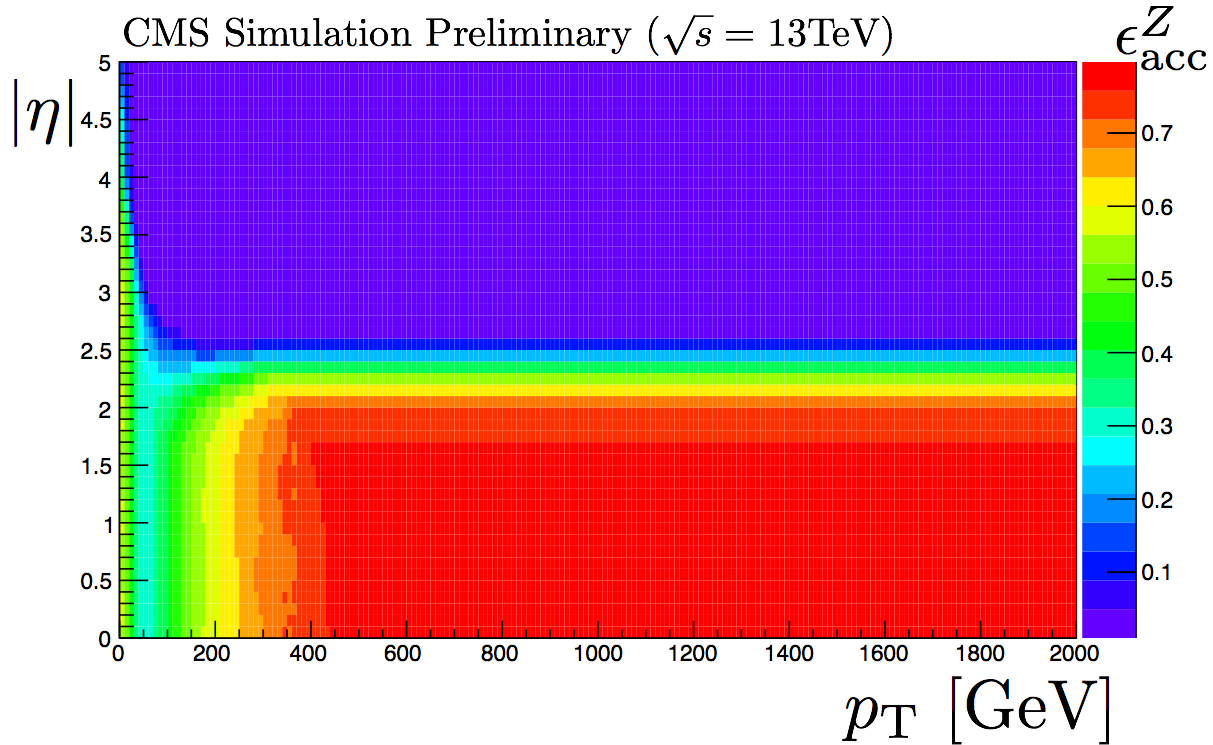
\includegraphics[width=0.7\linewidth]{figures/SusySearches/HadStop2015/ZeeAcceptance.png}
\caption{The $Z$ boson acceptance in simulated events with $\zee$.}
\label{fig:ZeeAcceptance}
\end{figure}

\subsubsection{Reconstruction efficiency $\epsilon^{\text{Z}}_{\text{rec}}$}
The reconstruction efficiency is defined as the fraction of $\zee$ events passing the acceptance criteria detailed in the previous section for which there are two reconstructed electrons in the event. The electron reconstruction is performed with the particle flow algorithm~{\cite{Beaudette:2014cea} introduced in Chapter \ref{chap:cms}. A set of selection criteria based on a recommendation by the Physics Object Group (POG) called the ``Cut Based VETO'' selection \cite{bib:ElectronID} is used, which features a very high overall electron efficiency of around 95\%. 

Since the reconstruction efficiency is expected to vary with the lepton $\pt$ and $\eta$, the $Z$ boson $\pt$ and $\eta$ are again selected as the observables used in the efficiency parametrization. Figure \ref{fig:ZeeReconstruction} shows the reconstruction efficiency as a function of the inferred $Z$ boson $\eta$ and $\pt$. 
\begin{figure}[tb!]
\centering
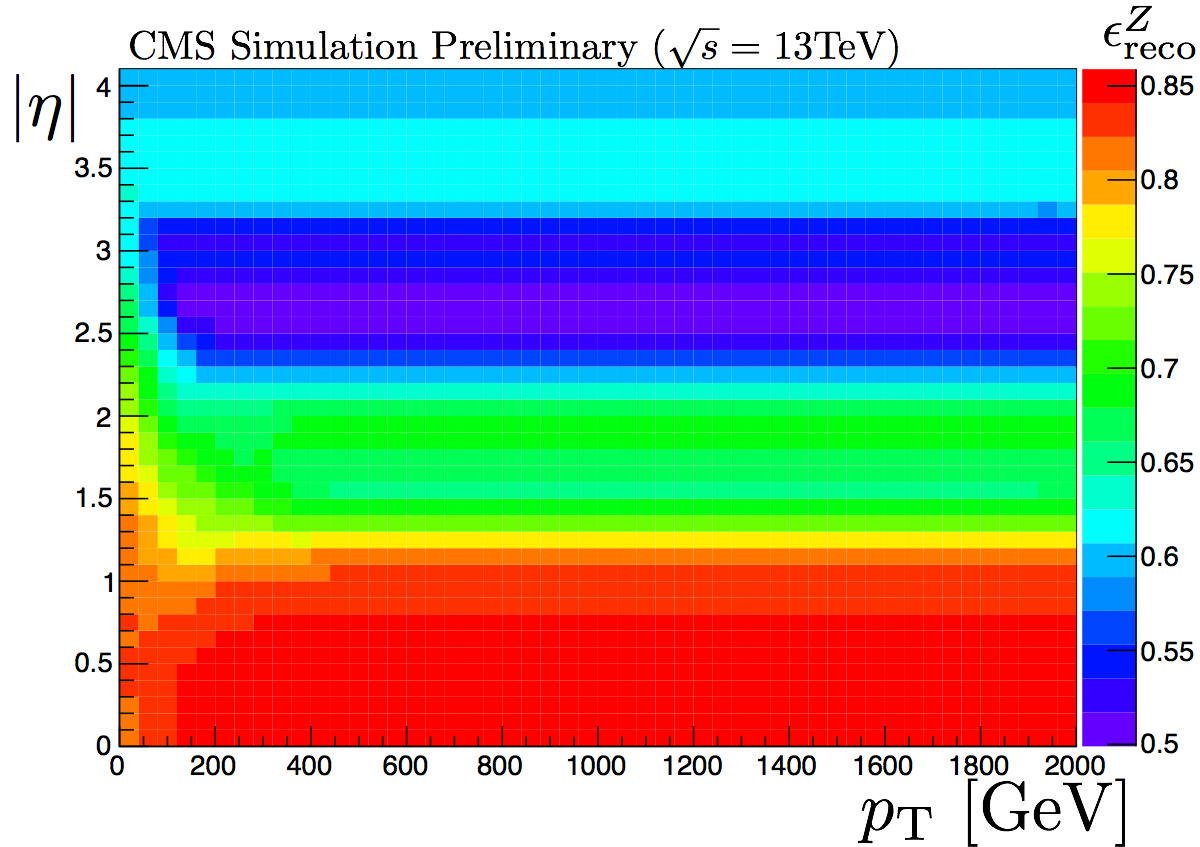
\includegraphics[width=0.7\linewidth]{figures/SusySearches/HadStop2015/ZeeReconstruction.png}
\caption{The $Z$ boson reconstruction efficiency in simulated events with $\zee$ decays.}
\label{fig:ZeeReconstruction}
\end{figure}
\FloatBarrier

\subsubsection{Isolation efficiency $\epsilon^{\text{Z}}_{\text{iso}}$}
The isolation efficiency is the fraction of $\zee$ events passing the acceptance and reconstruction criteria detailed in the previous sections for which there are two isolated electrons in the event. 

Unlike for the acceptance and the reconstruction efficiency, the isolation of the electrons is not strongly correlated with the $\pt$ or $\eta$ of the parent $Z$ boson, at least for Z $\pt$ less than 300 GeV. Observables that describe the $Z$ boson, but which are correlated with the electron isolation, must be constructed. There are two main effects that can cause an event to fail the isolation: first, one or both of the electrons may happen to travel in a direction collinear with jets or other particles in the event. Second, in the case of a highly energetic $Z$ boson, the electrons can be highly collinear with each other. It makes sense to parametrize the efficiency as a function of one variable that captures the effects of the first scenario, and one variable that captures those of the second. The variables chosen are the $\Delta R (\text{e}_1, \text{e}_2)$ between the two electrons, and the geometric mean of the activity of the two electrons, where the activity is defined as the $\pt$ sum of reconstructed particles in an annulus around the lepton in the $\eta-\phi$ plane with an inner radius of the isolation cone radius and an outer radius of 0.4, divided by the lepton $\pt$:

\begin{equation}
\text{activity} = \sum_{i}(p_{T})_i \cdot \Theta[0.4-\Delta R_{i})] \cdot \Theta[\Delta R_{i}-R^*]/(p_T)_{\text{lepton}},
\end{equation}
where R$^*$ is defined above.
Figure \ref{fig:ZeeIsolation} shows the isolation efficiency map using this parametrization. 
\begin{figure}[tb!]
\centering
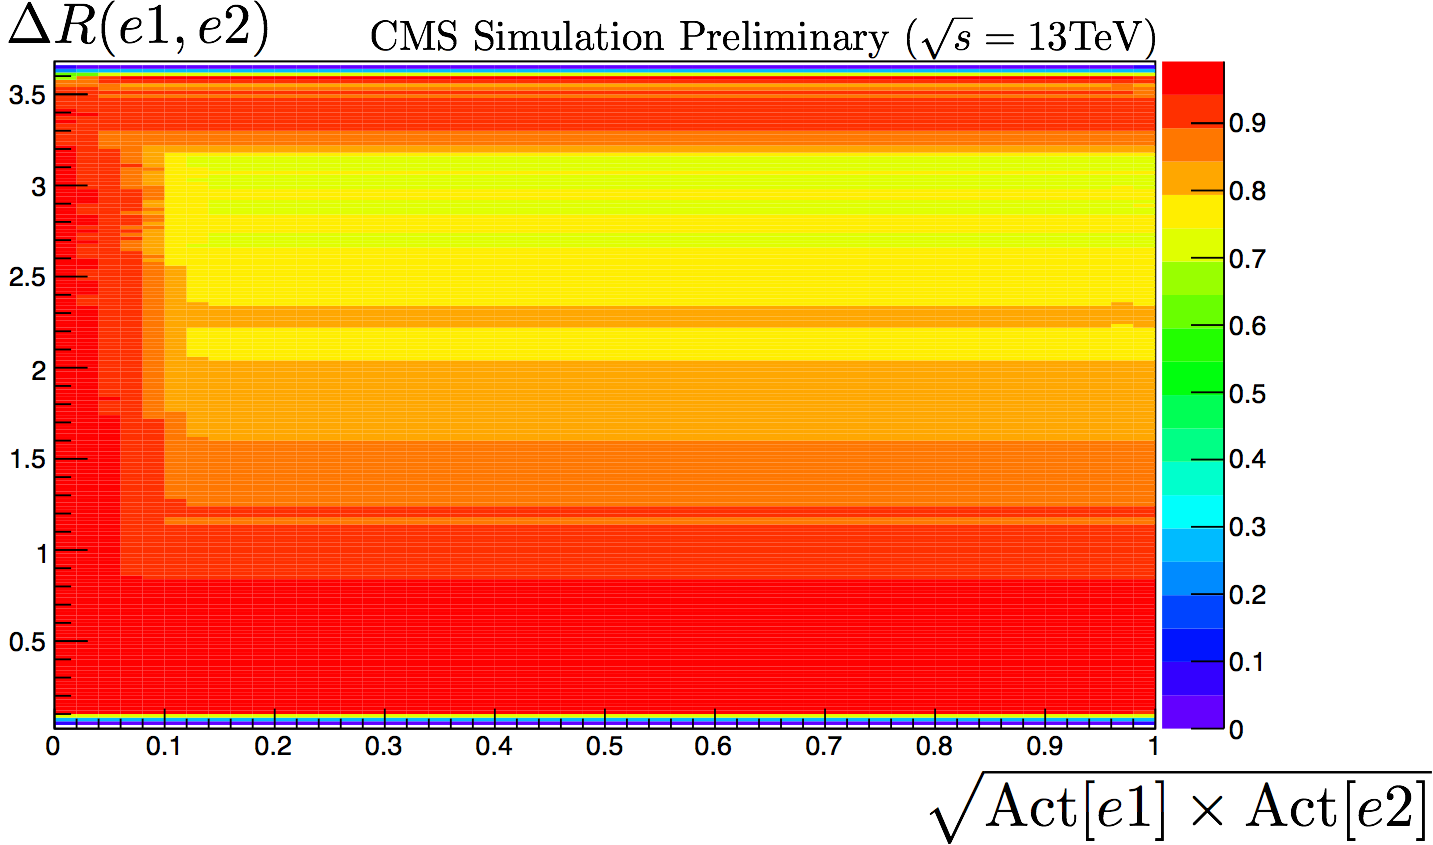
\includegraphics[width=0.7\linewidth]{figures/SusySearches/HadStop2015/ZeeIsolation.png}
\caption{The $Z$ boson isolation efficiency as a function of the $\Delta R$ between the two electrons and the geometric mean of the activities of the electrons in simulated events with $\zee$ decays.}
\label{fig:ZeeIsolation}
\end{figure}
\FloatBarrier

\subsection{Closure}
The prediction is applied to simulated $\zll$ events and compared with the result obtained directly from $\zinv$ simulation. The baseline selection of \cite{Khachatryan:2016kdk}, 
\begin{itemize}
\item no reconstructed, isolated lepton with a $\pt>10$ GeV and $|\eta|<2.4$;
\item no reconstructed, isolated particle track with a $\pt>10$ GeV and $|\eta|<2.4$;
\item $\Ht>500$ GeV;
\item $\met>200$ GeV;
\item $\Delta\phi(\mht$, jet$_{1,2,3})>$ 0.5, 0.5, 0.3;
\item $N_t\geq1$, where $N_t$ is the multiplicity of jets identified as originating from a top quark;
\item $\nbjets\geq1$, and
\item $M_{\text{T2}}>200$ GeV (see Appendix \ref{app:discriminators} for more details).
\end{itemize}
described in greater detail in the Section \ref{sec:2015results}}, is applied. Figures \ref{fig:ZInvBaseline_MetHtNjMt2} and \ref{fig:ZInvBaseline_NbNt} show the distributions for the $\zinv$ prediction using Equation \ref{eq:zinv}, the efficiencies presented in the previous section, the branching fractions quoted in Table \ref{tab:zdecay}, compared with the expectation from $\zinv$ simulation. Figures \ref{fig:ZInvCR_MetHtNjMt2} and \ref{fig:ZInvCR_NbNt} show the comparisons in the loosened baseline control region (also described in Section~\ref{sec:2015results}) in which the $\met$ and $\Ht$ selection has been relaxed.
\begin{figure}[tb!]
\centering
\subfloat[]{
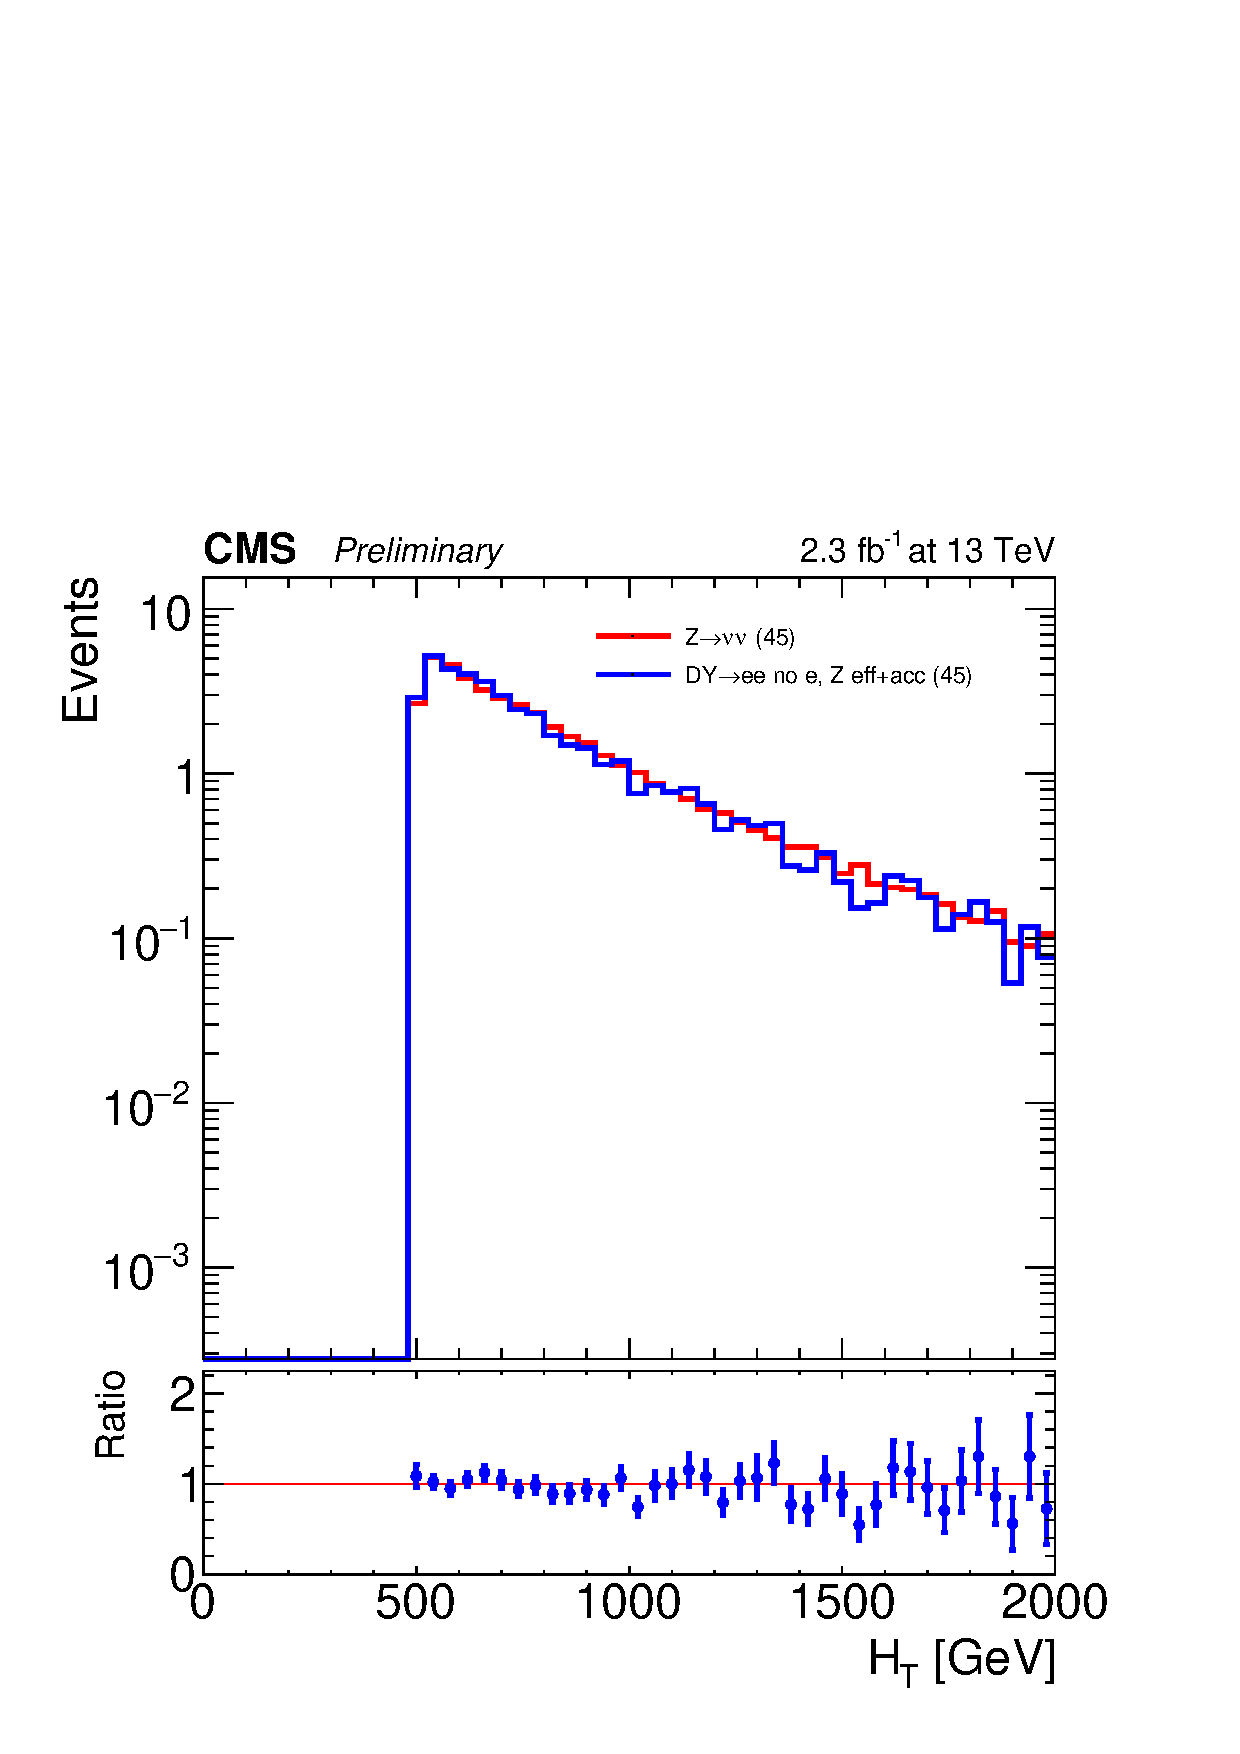
\includegraphics[width=0.5\linewidth]{figures/SusySearches/HadStop2015/MCClosure_elec_baseline_cleanht.pdf}
}
\subfloat[]{
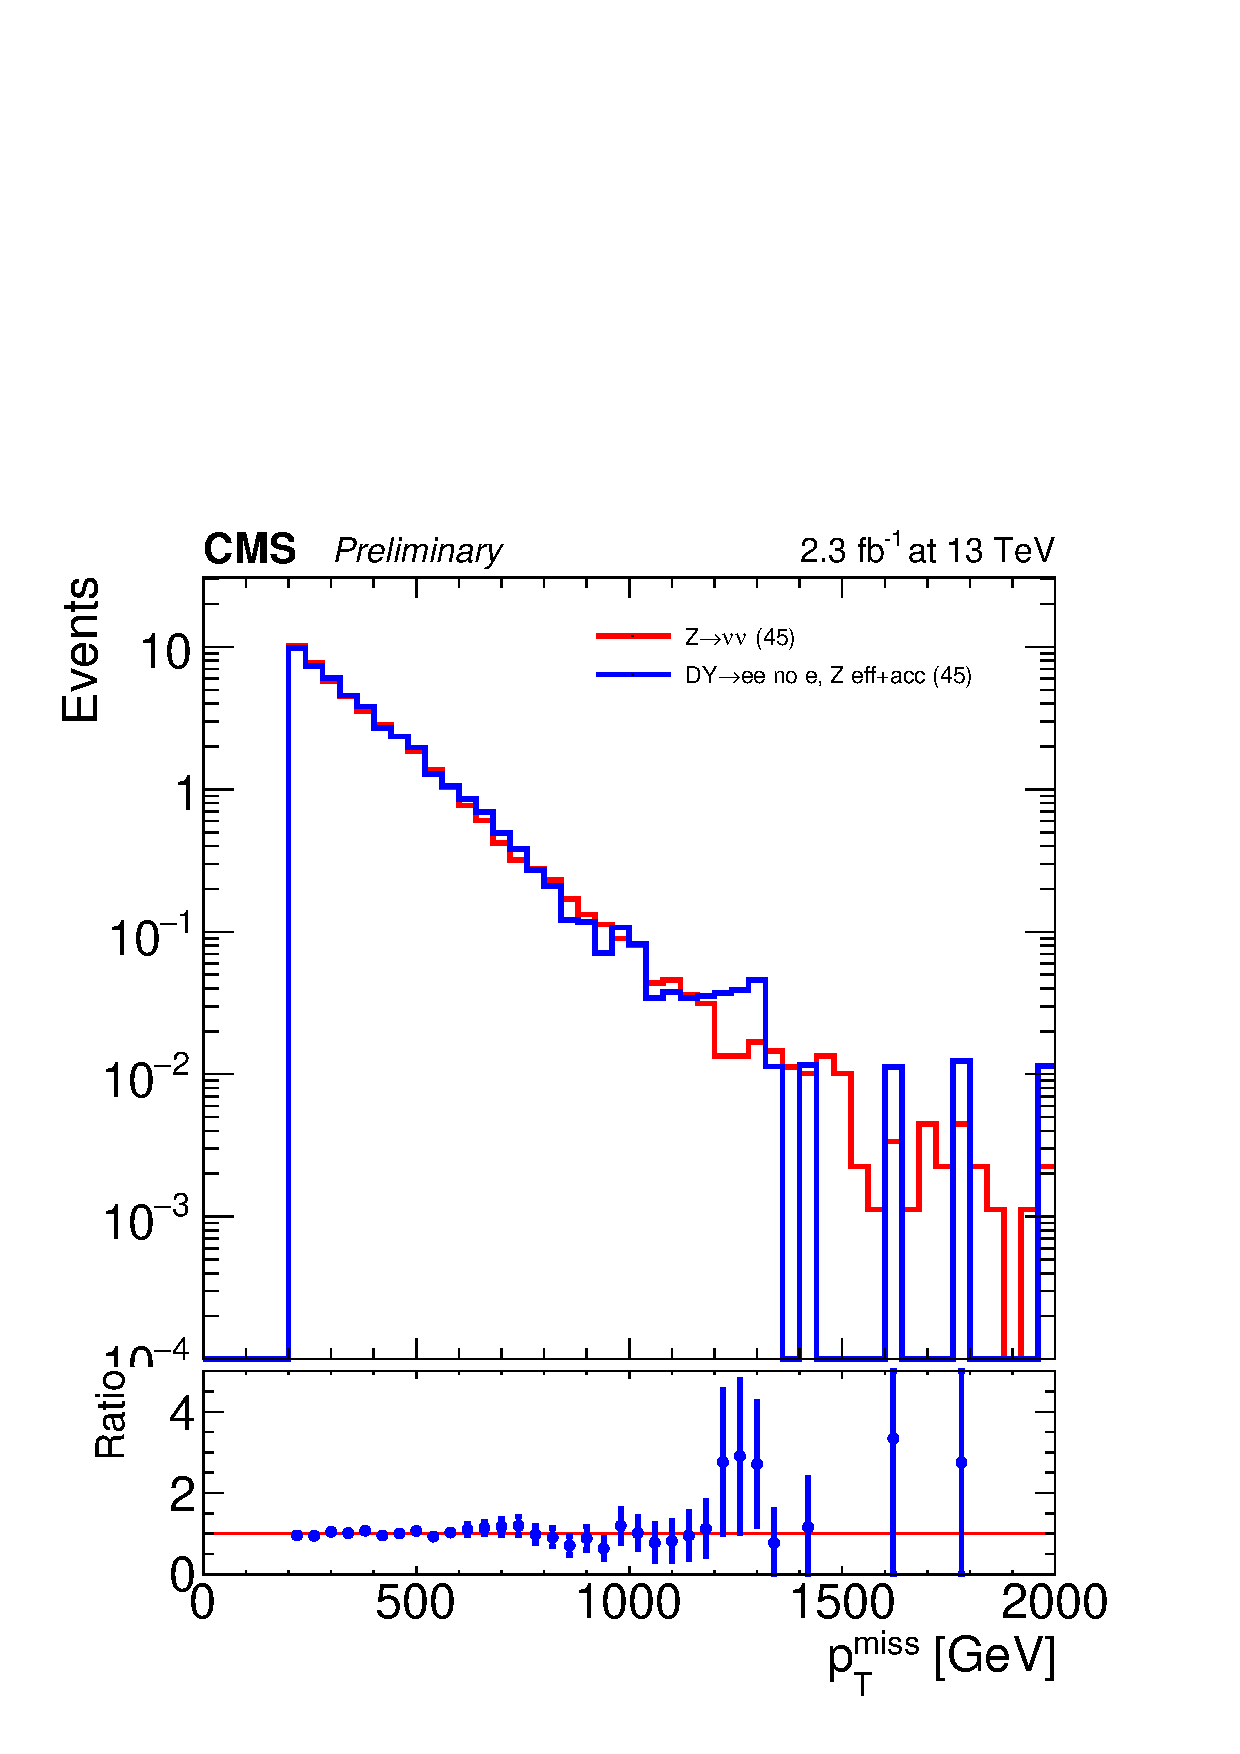
\includegraphics[width=0.5\linewidth]{figures/SusySearches/HadStop2015/MCClosure_elec_baseline_cleanmet.pdf}
}\\
\subfloat[]{
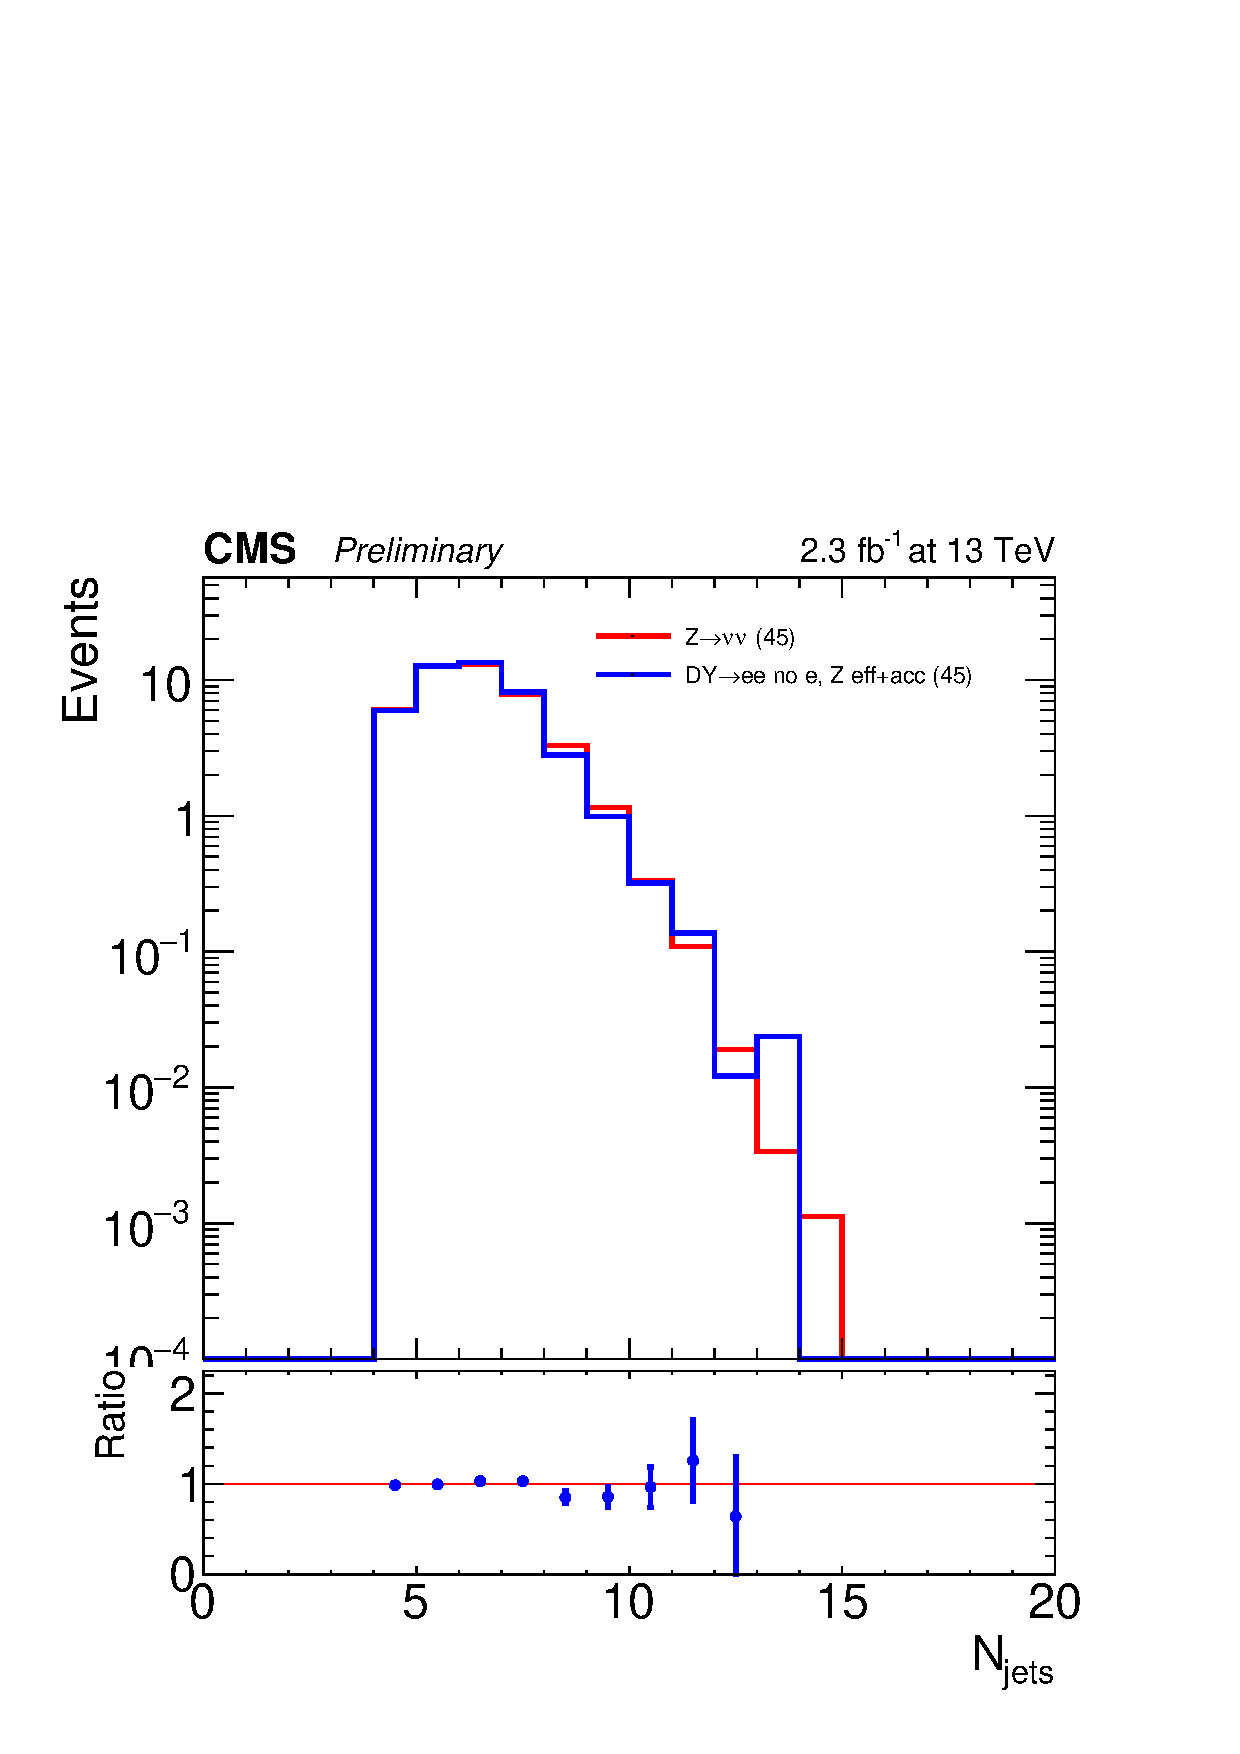
\includegraphics[width=0.5\linewidth]{figures/SusySearches/HadStop2015/MCClosure_elec_baseline_cleannJet.pdf}
}
\subfloat[]{
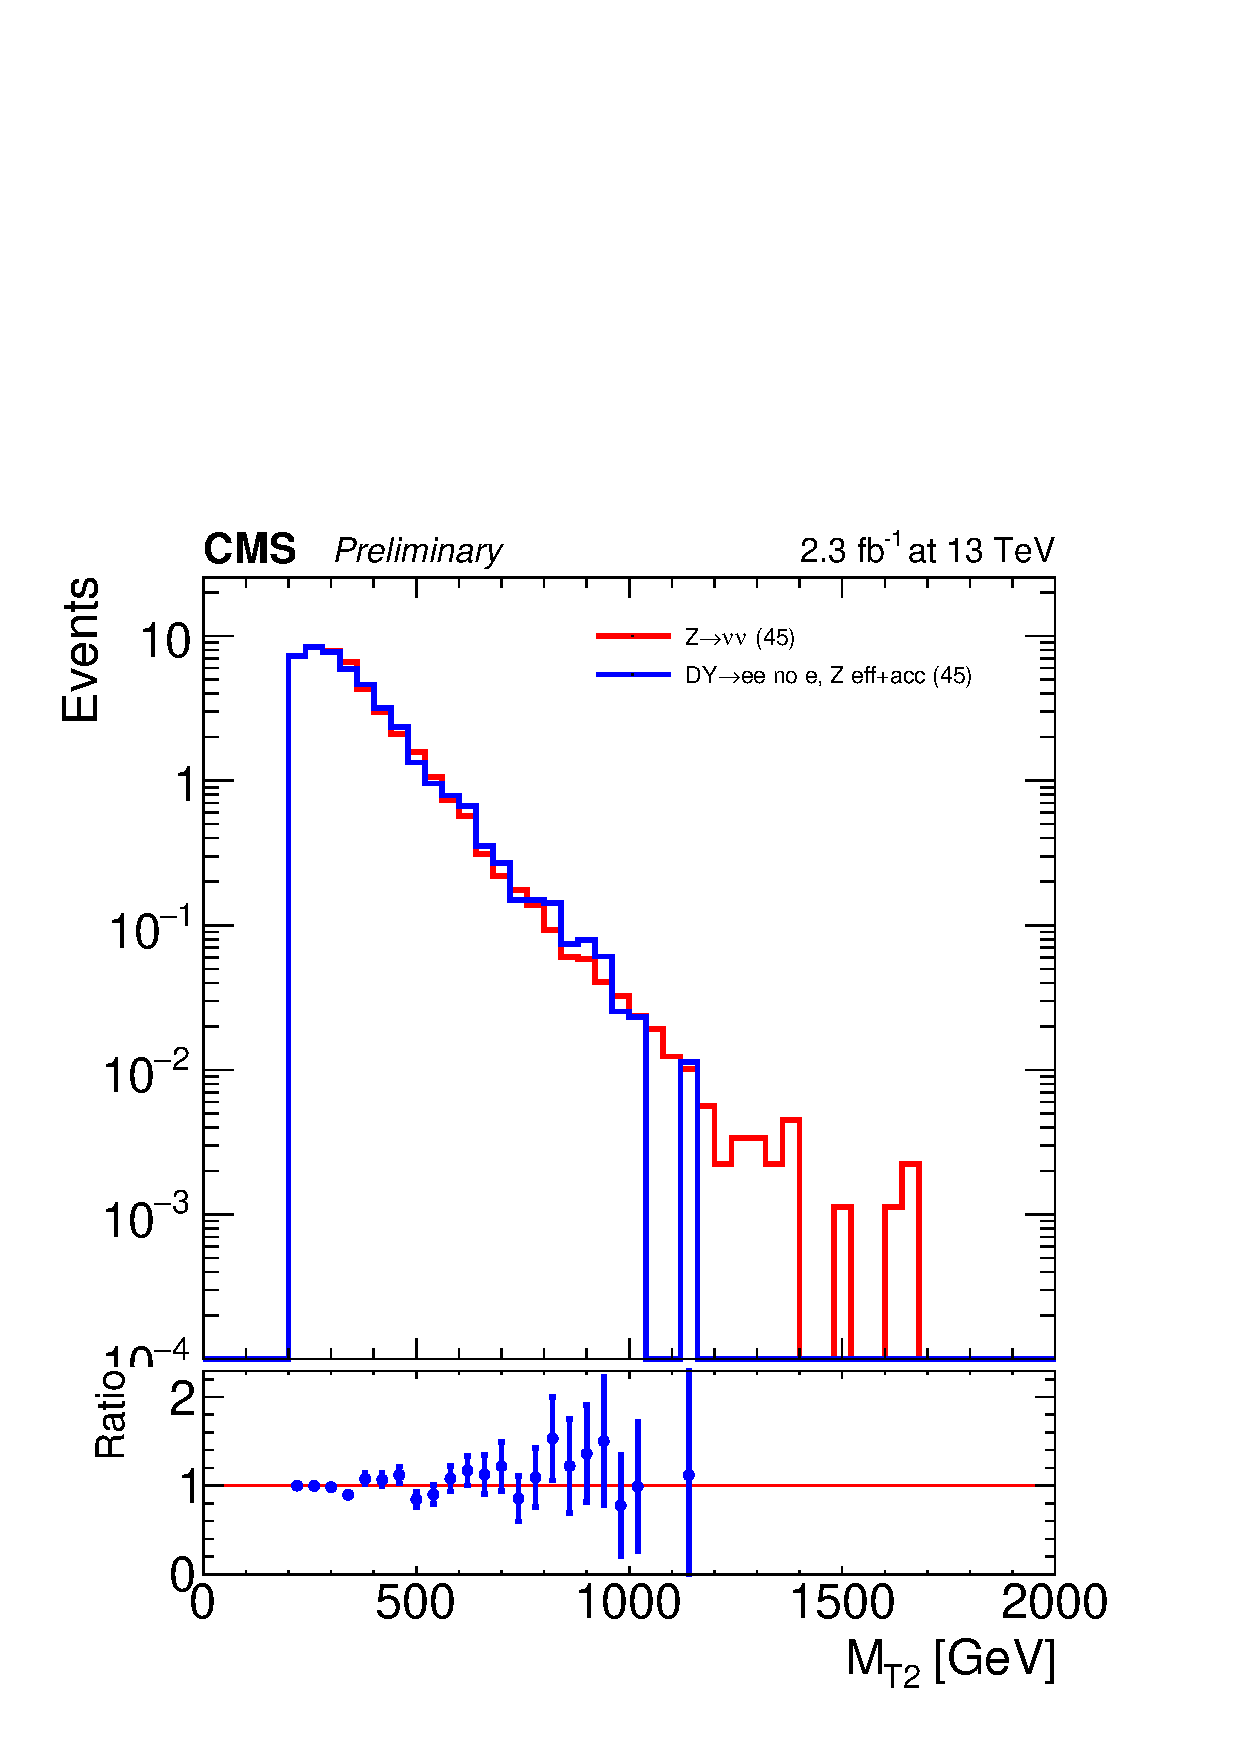
\includegraphics[width=0.5\linewidth]{figures/SusySearches/HadStop2015/MCClosure_elec_baseline_mT2Zinv.pdf}
}
\caption{Comparison of $\zinv$ prediction (blue) and expectation (red) for the $\Ht$ (1) and $\met$ (2), the jet multiplicity (3) and the $M_{T2}$ (4), after the baseline selection of the 2015 hadronic stop analysis. The ratio is of the prediction to the expectation. All events are from simulation.}
\label{fig:ZInvBaseline_MetHtNjMt2}
\end{figure}

\begin{figure}[tb!]
\centering
\subfloat[]{
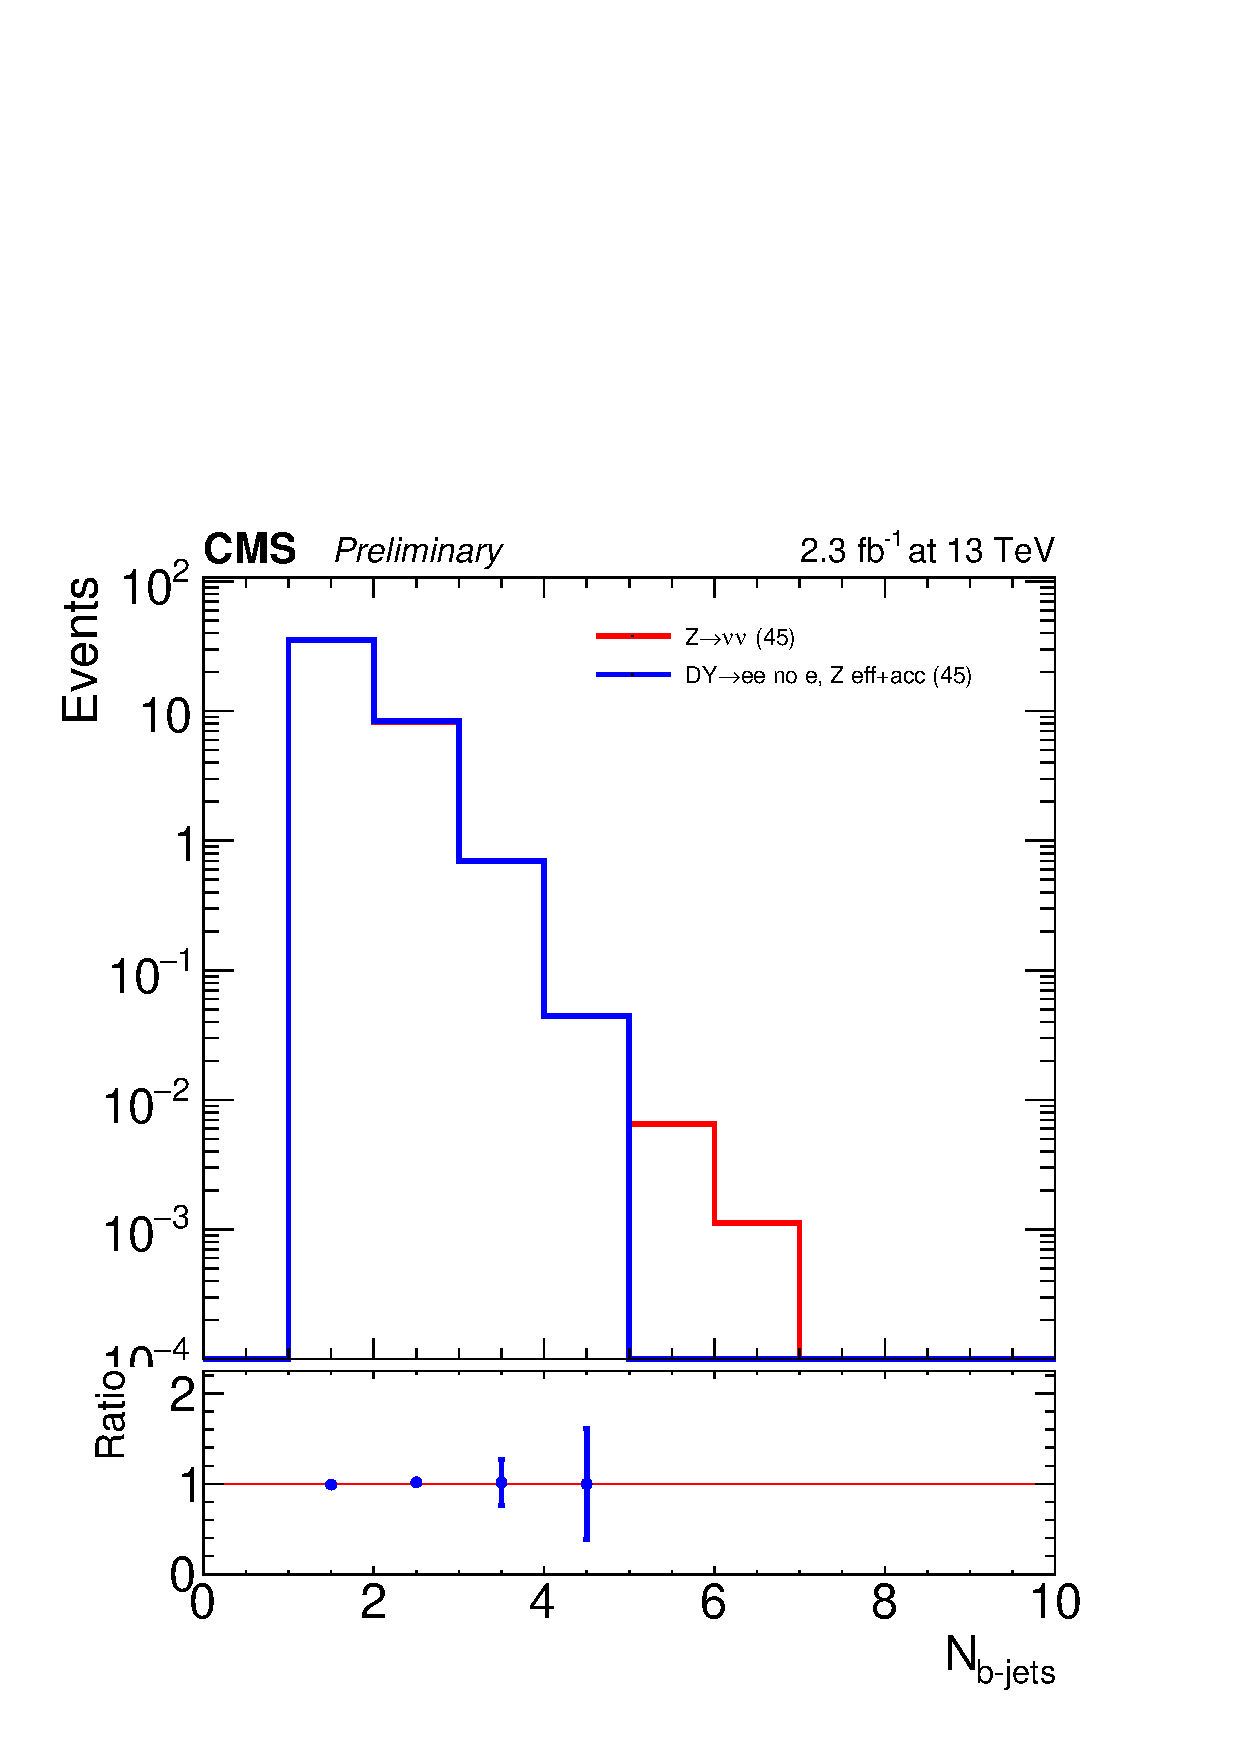
\includegraphics[width=0.5\linewidth]{figures/SusySearches/HadStop2015/MCClosure_elec_baseline_nBottom.pdf}
}
\subfloat[]{
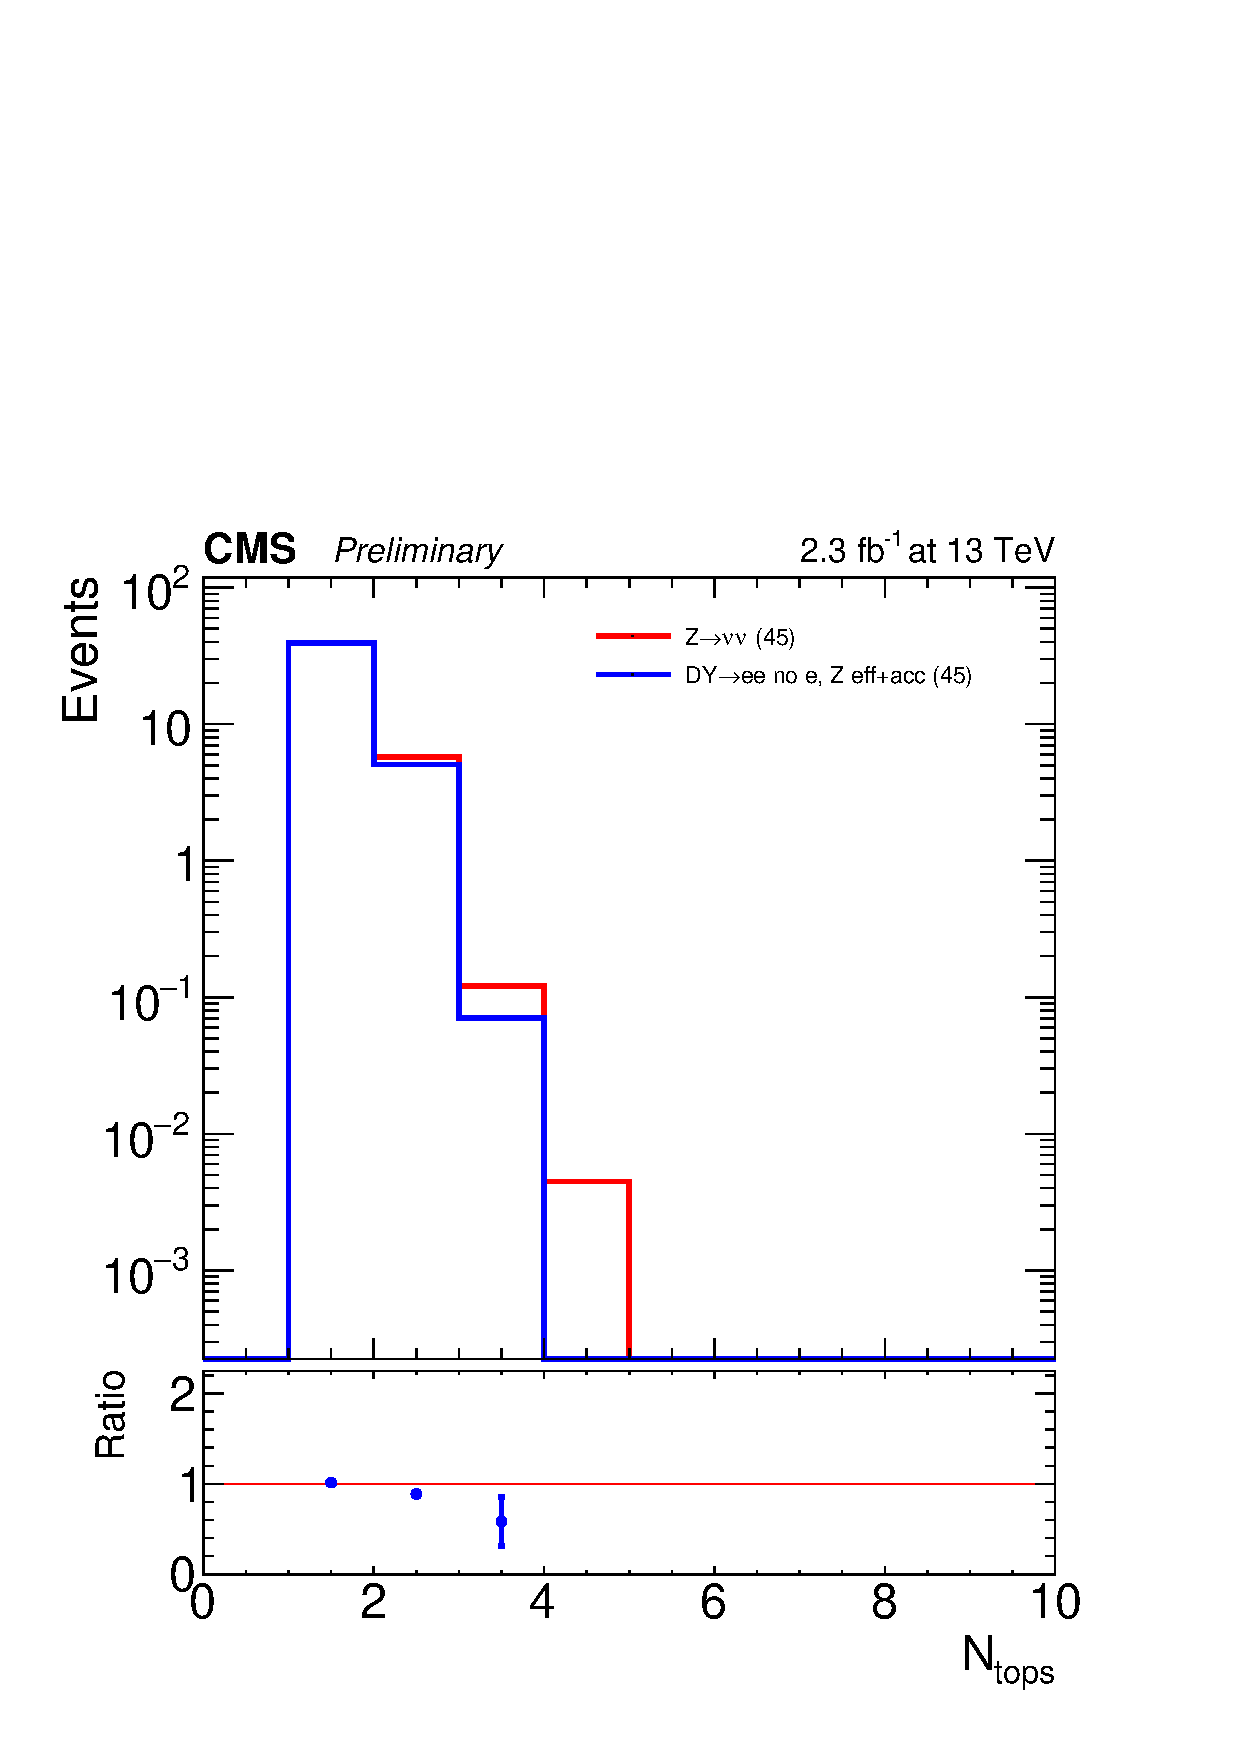
\includegraphics[width=0.5\linewidth]{figures/SusySearches/HadStop2015/MCClosure_elec_baseline_nTop.pdf}
}
\caption{Comparison of $\zinv$ prediction (blue) and expectation (red) for the b-jet multiplicity (1) and top tag multiplicity (2), after the baseline selection of the 2015 hadronic stop analysis. The ratio is of the prediction to the expectation. All events are from simulation.}
\label{fig:ZInvBaseline_NbNt}
\end{figure}
\begin{figure}[tb!]
\centering
\subfloat[]{
\includegraphics[width=0.5\linewidth]{figures/SusySearches/HadStop2015/ZinvEle_LooseHt.pdf}
}
\subfloat[]{
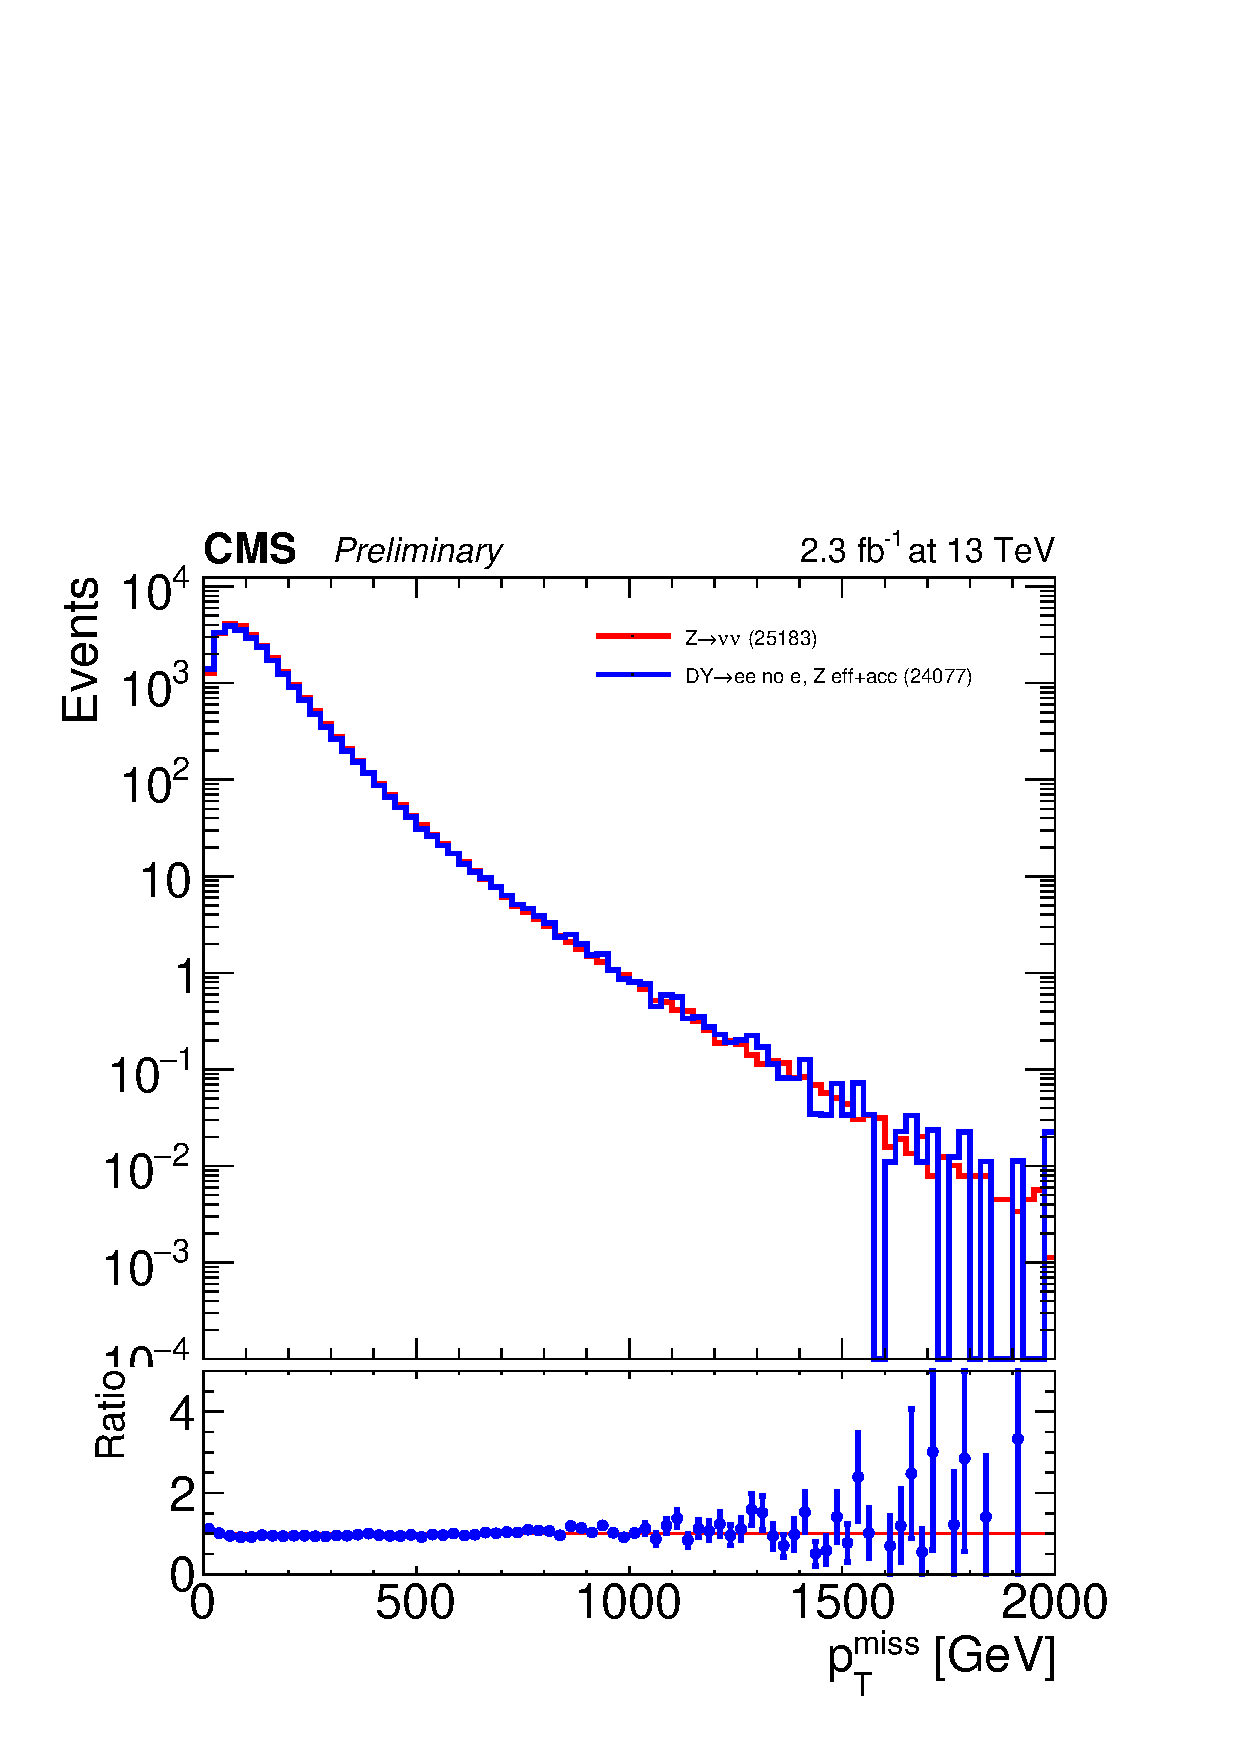
\includegraphics[width=0.5\linewidth]{figures/SusySearches/HadStop2015/ZinvEle_LooseMet.pdf}
}\\
\subfloat[]{
\includegraphics[width=0.5\linewidth]{figures/SusySearches/HadStop2015/ZinvEle_LooseNj.pdf}
}
\subfloat[]{
\includegraphics[width=0.5\linewidth]{figures/SusySearches/HadStop2015/ZinvEle_LooseMt2.pdf}
}
\caption{Comparison of $\zinv$ prediction (blue) and expectation (red) for the $\Ht$ (1) and $\met$ (2), the jet multiplicity (3) and the $M_{T2}$ (4), after a loosened baseline selection for the 2015 hadronic stop analysis. The ratio is of the prediction to the expectation. All events are from simulation.}
\label{fig:ZInvCR_MetHtNjMt2}
\end{figure}

\begin{figure}[tb!]
\centering
\subfloat[]{
\includegraphics[width=0.5\linewidth]{figures/SusySearches/HadStop2015/ZinvEle_LooseNb.pdf}
}
\subfloat[]{
\includegraphics[width=0.5\linewidth]{figures/SusySearches/HadStop2015/ZinvEle_LooseNt.pdf}
}
\caption{Comparison of $\zinv$ prediction (blue) and expectation (red) for the b-jet multiplicity (1) and top tag multiplicity (2), after the loosened baseline selection for the 2015 hadronic stop analysis. The ratio is of the prediction to the expectation. All events are from simulation.}
\label{fig:ZInvCR_NbNt}
\end{figure}
\noindent
The prediction and expectation agree to within a few percent across all distributions, indicating the soundness of the method; in other words, the method closes. I note that the closure holds in the region of low to moderate $\met$, where it was previously determined that large nonexcluded SUSY signals could be manifest (see Chapter \ref{chap:run1pmssm}), and which will be considered in Chapter \ref{chap:money}. The method is now at a stage where it can be applied in a fully data-driven prediction. 

\FloatBarrier
\subsection{Applying the method in data}
The final $\zinv$ prediction used in \cite{CMS:2016nhb} relies on a reweighting of simulated $\zinv$ events to account for differences between data and simulation. Weights are derived in bins of $\njets$ and $\nbjets$ by dividing the counts observed in a real dilepton data sample, which has been treated with the data-driven background estimation (Equation \ref{eq:zinv}), by the counts predicted directly by $\zinv$ simulation, after a loosened baseline selection has been applied. The loose selection is defined similarly to the baseline selection, but with
\begin{itemize}
\item $\Ht>200$ GeV;
\item $\met>0$ GeV;
\item $\mttwo>0$ GeV;
\end{itemize}

The weights derived from the ee sample are compared with those based on the $\mu\mu$ sample in Fig. \ref{fig:ZInvWeights}. 
\begin{figure}[tb!]
\centering
\subfloat[]{
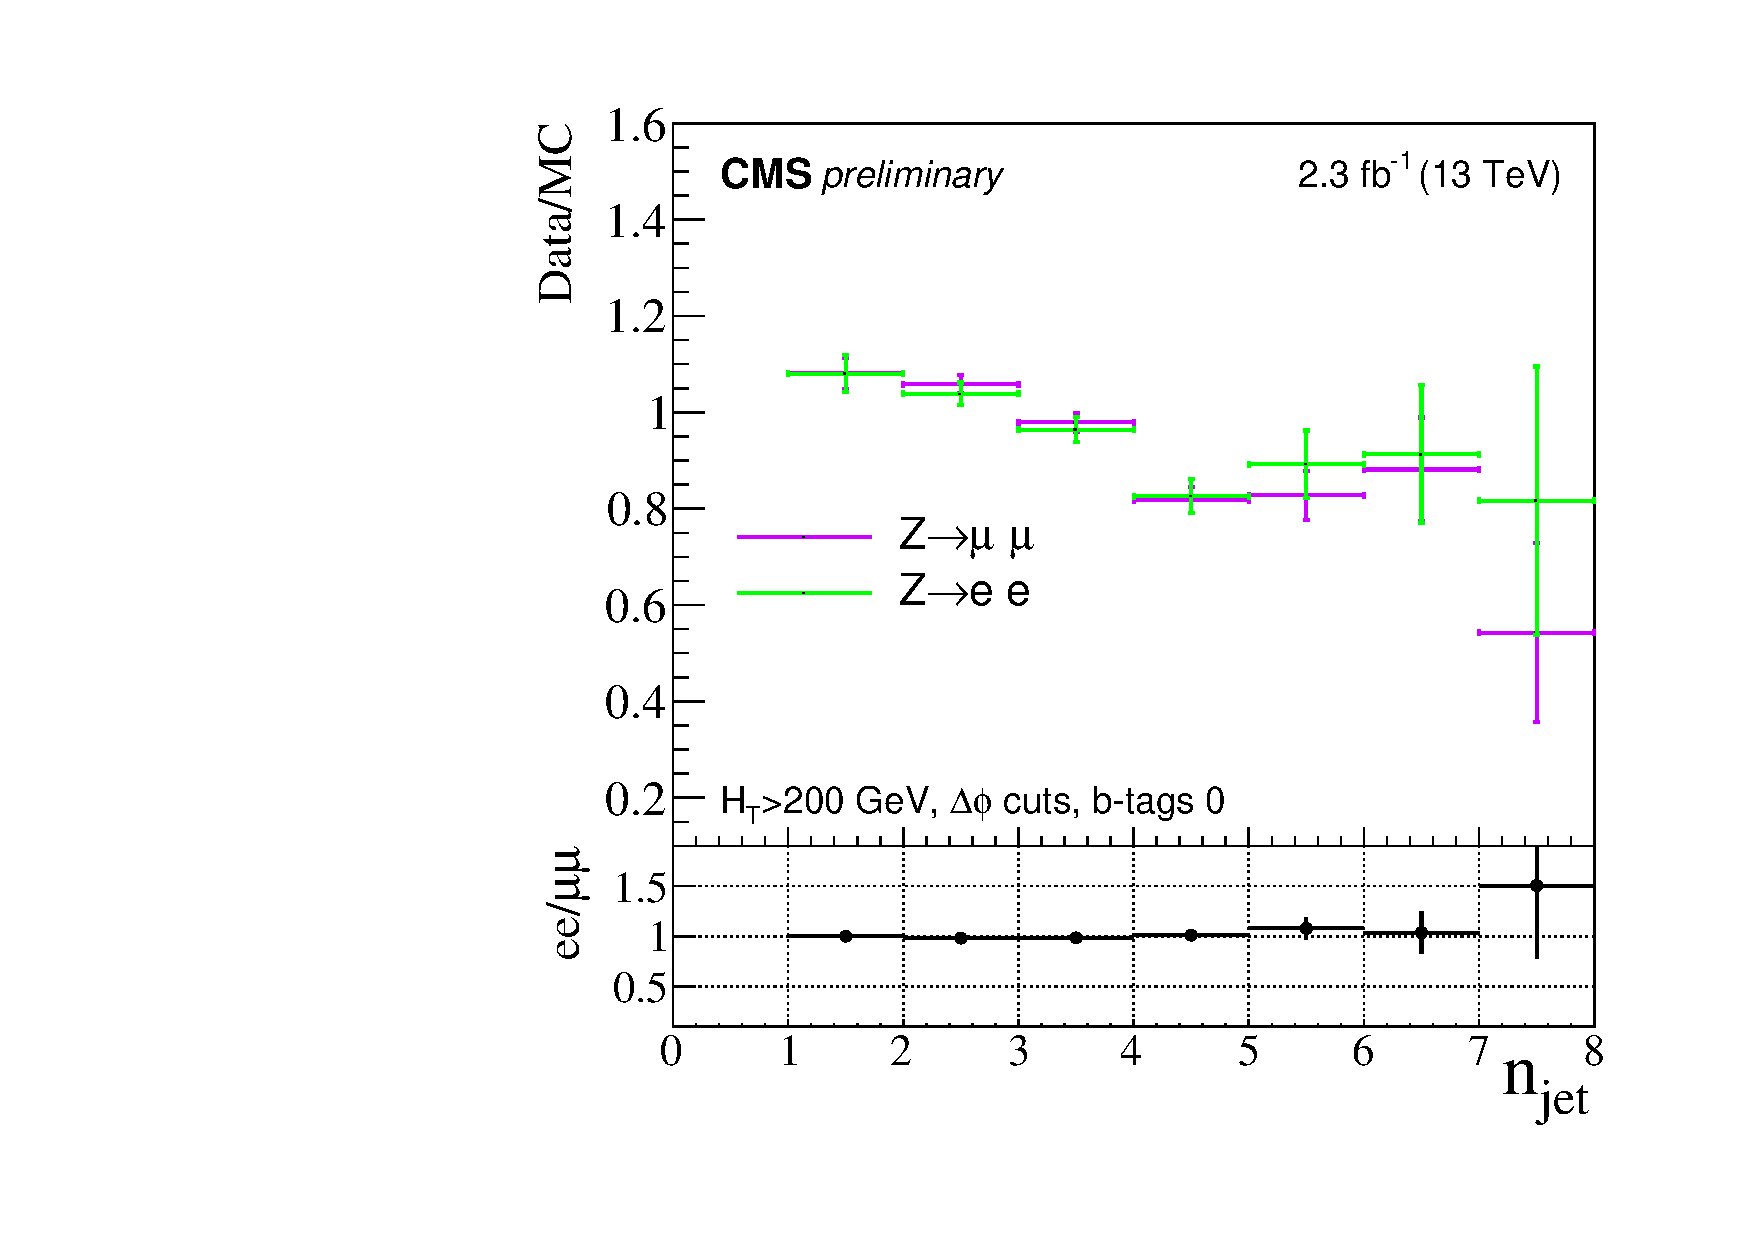
\includegraphics[width=0.5\linewidth]{figures/SusySearches/HadStop2015/NJetWeightElVsMu_0b.pdf}
}
\subfloat[]{
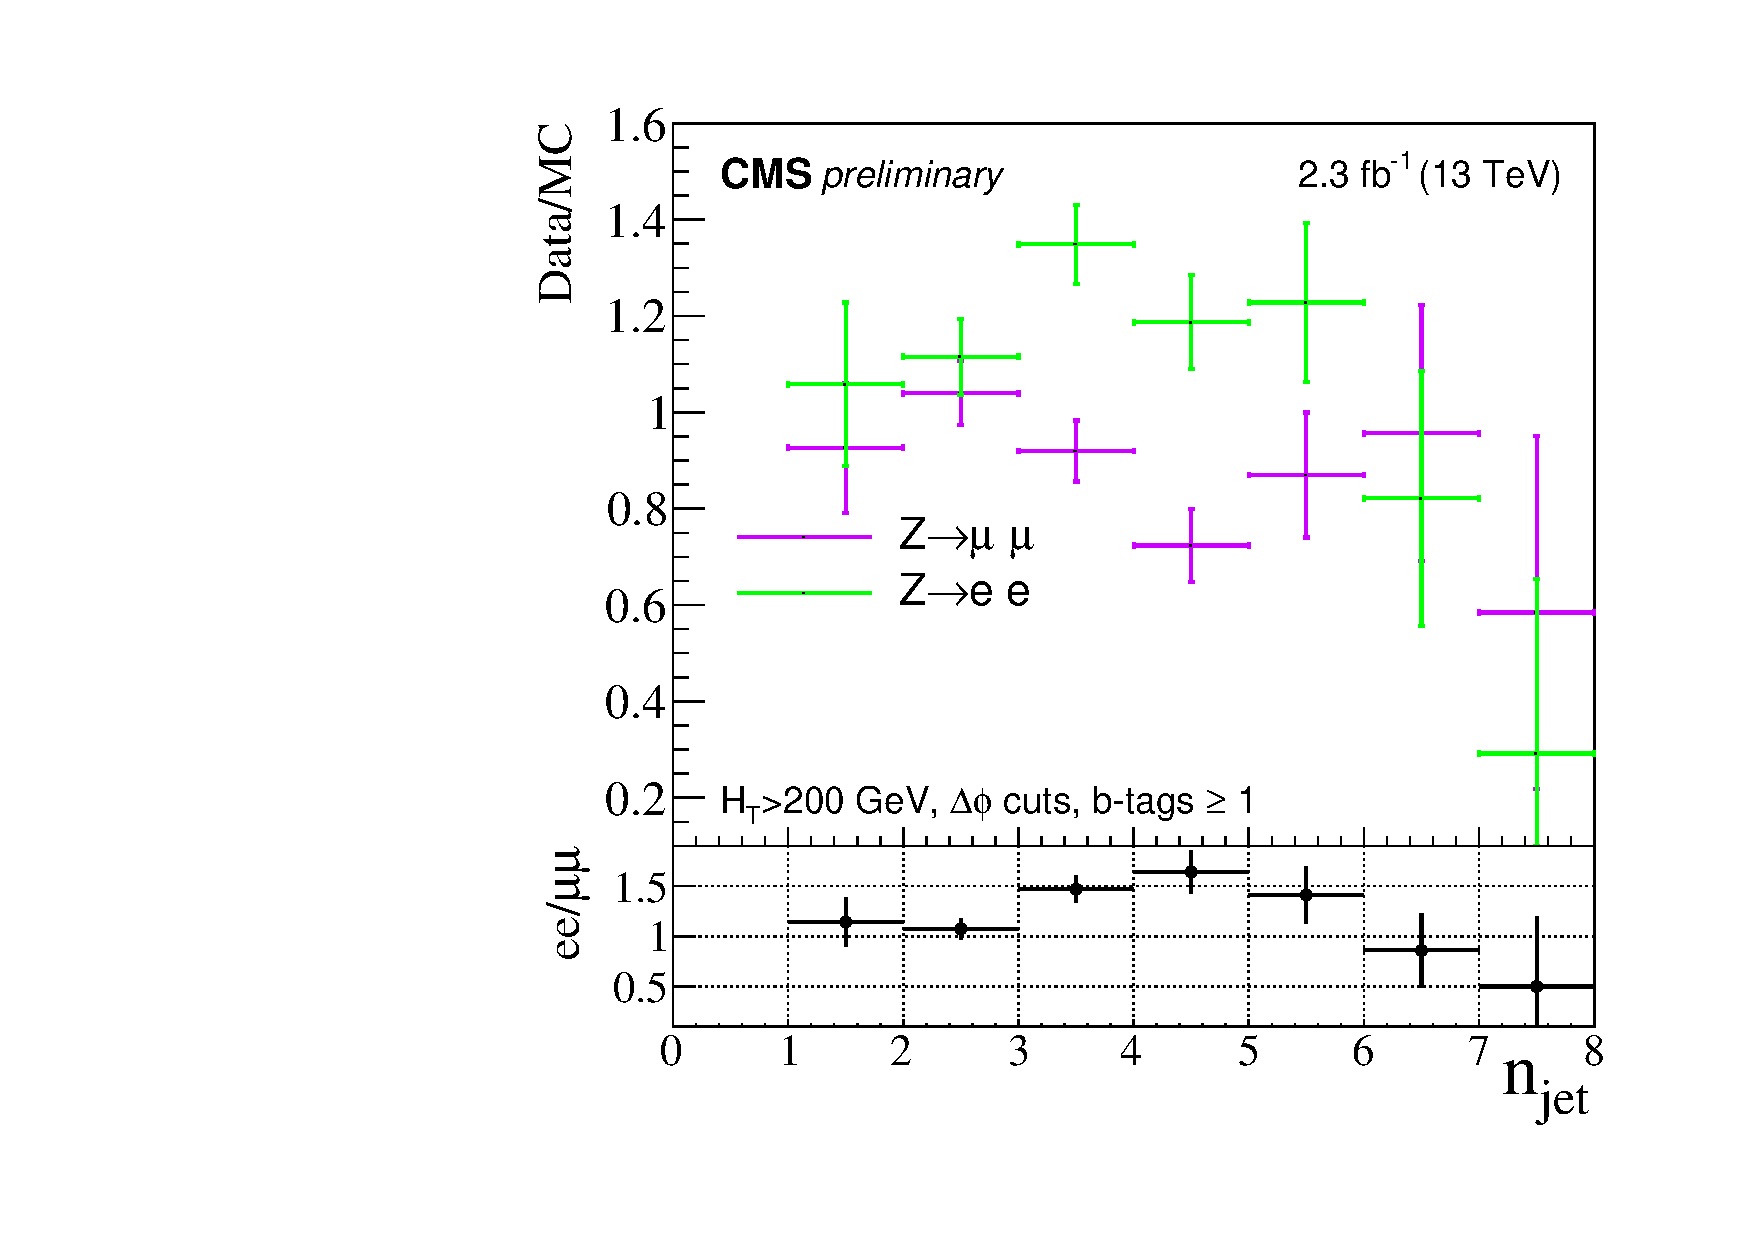
\includegraphics[width=0.5\linewidth]{figures/SusySearches/HadStop2015/NJetWeightElVsMu_1b.pdf}
}
\caption{Comparison of data/simulation event weights for the $\zinv$ prediction based on the electron sample (green) and the muon sample (magenta) for the b-jet multiplicity 0 (left) b-jet multiplicity greater than 0 (right), after the loosened baseline selection for the 2015 hadronic stop analysis. The denominator of the weights are the counts taken from on $\zll$ simulation, and the numerator is the count in $\zll$ data where the t$\bar{\text{t}}$ contribution has been subtracted using simulation. }
\label{fig:ZInvWeights}
\end{figure}
For events with no b-tagged jets, the weights from the ee and $\mu\mu$ sample agree within the statistical uncertainties. For events with one or more b-tagged jet, at least one bin of jet multiplicity shows a noticeable departure between the two methods. It remains to be determined if this effect is statistical in nature, or if it represents a systematic difference between the electron and muon methods. Examination of the data collected in 2016 will play an important role in answering this question.

An overall simulation-to-data normalization factor is derived in a control region with 0 b-tagged jets and applied to the $\zinv$ simulation as part of the final prediction. A comparison of the normalization factor derived from the ee sample with that derived from the $\mu\mu$ sample is shown in Fig. \ref{fig:ZInvNorm}.
\begin{figure}[tb!]
\centering
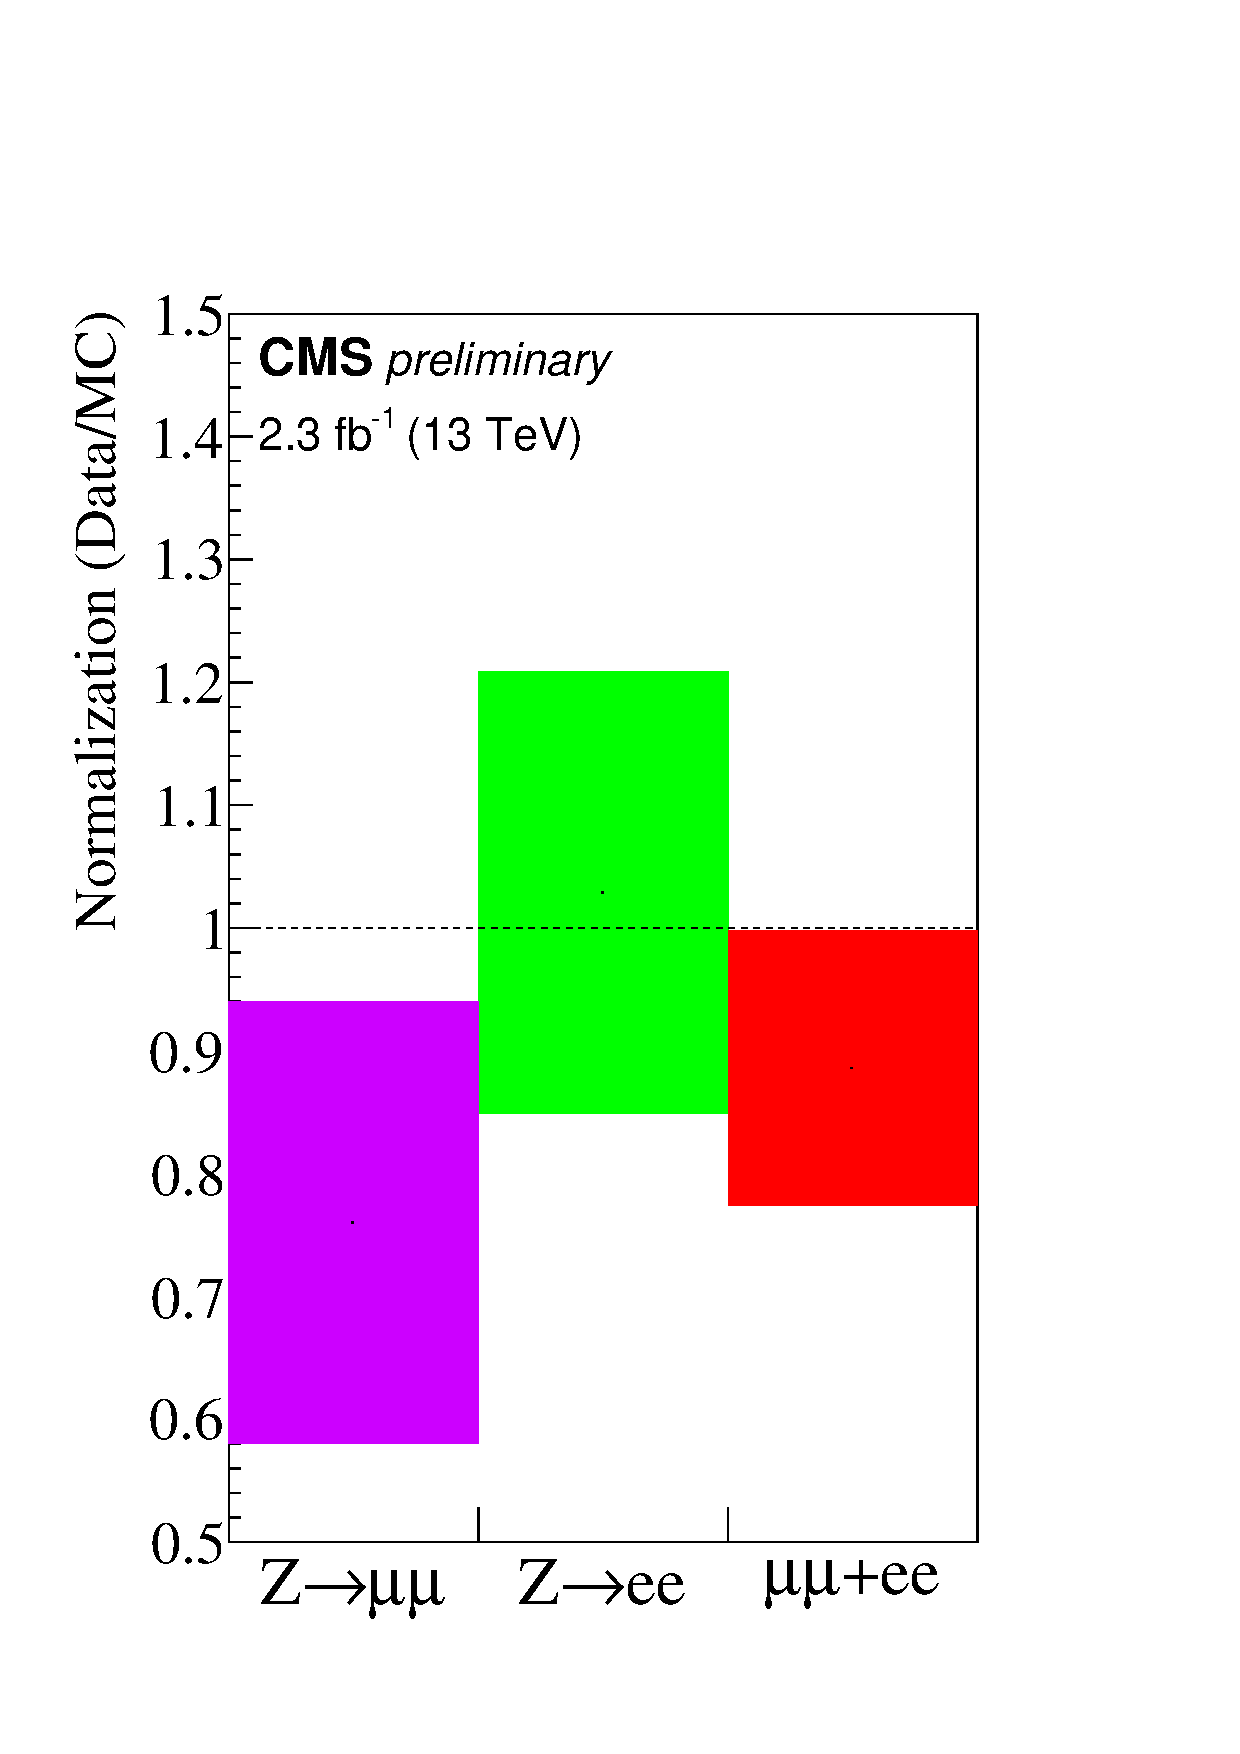
\includegraphics[width=0.4\linewidth]{figures/SusySearches/HadStop2015/NormFactors.pdf}
\caption{The data-simulation normalization factor computed from the $\mu\mu$ sample (magenta), the ee sample (green), and the combined ee $+$ $\mu\mu$ sample (red). }
\label{fig:ZInvNorm}
\end{figure}
\noindent
The electron- and muon-derived normalization factors agree within statistical uncertainties, indicating that a trivial combination of the electron and muon data is justifiable in the derivation of the normalization factor and its uncertainty. After combining the electron and muon prediction samples, the systematic uncertainty in the $\zinv$ prediction associated with the normalization is reduced by approximately 30\%. Uncertainties are discussed now.

\FloatBarrier
\subsection{Uncertainties in the prediction}
Uncertainties in the $\zinv$ prediction include the statistical uncertainty of the simulated samples, uncertainty in the normalization, uncertainty associated with differences between real and simulated data, the statistical uncertainty in the $\njets-\nbjets$ weights, and other small uncertainties related to jet energy, $\met$, factorization scale, and PDFs.  

The statistical uncertainty in the prediction is the bin-by-bin poisson uncertainty in the weighted simulated $\zinv$ counts. These uncertainties are negligible for the analysis \cite{CMS:2016nhb}.

The statistical uncertainty in the normalization, as well as uncertainties in the $\njets-\nbjets$ weights, are propagated to the signal region, and treated as correlated across all search regions.

Uncertainties associated with the differences in the shapes of simulated and real distributions are computed bin-by-bin in the so-called loose $N_{\text{top}}$ region, defined analogously to the baseline selection but with no criterion placed on the multiplicity of top-tagged jets. For each search bin, four comparisons are made between the data and reweighted simulated counts, one for each of the four observables, $\met$, $\mttwo$, $\nbjets$, and $N_{\text{top}}$. All but the observable considered are integrated over their full ranges, and the observable considered is integrated over the values set by the search bin for that observable. The maximum discrepancy among the four comparisons is taken as a percent uncertainty in the predicted $\zinv$ count in the bin. Comparisons of dilepton data, treated with the data-driven method, and reweighted simulation are shown in Fig. \ref{fig:zinvdatamc}. Uncertainties are taken to be uncorrelated across bins.


\begin{figure}[tb!]
\centering
\subfloat[]{
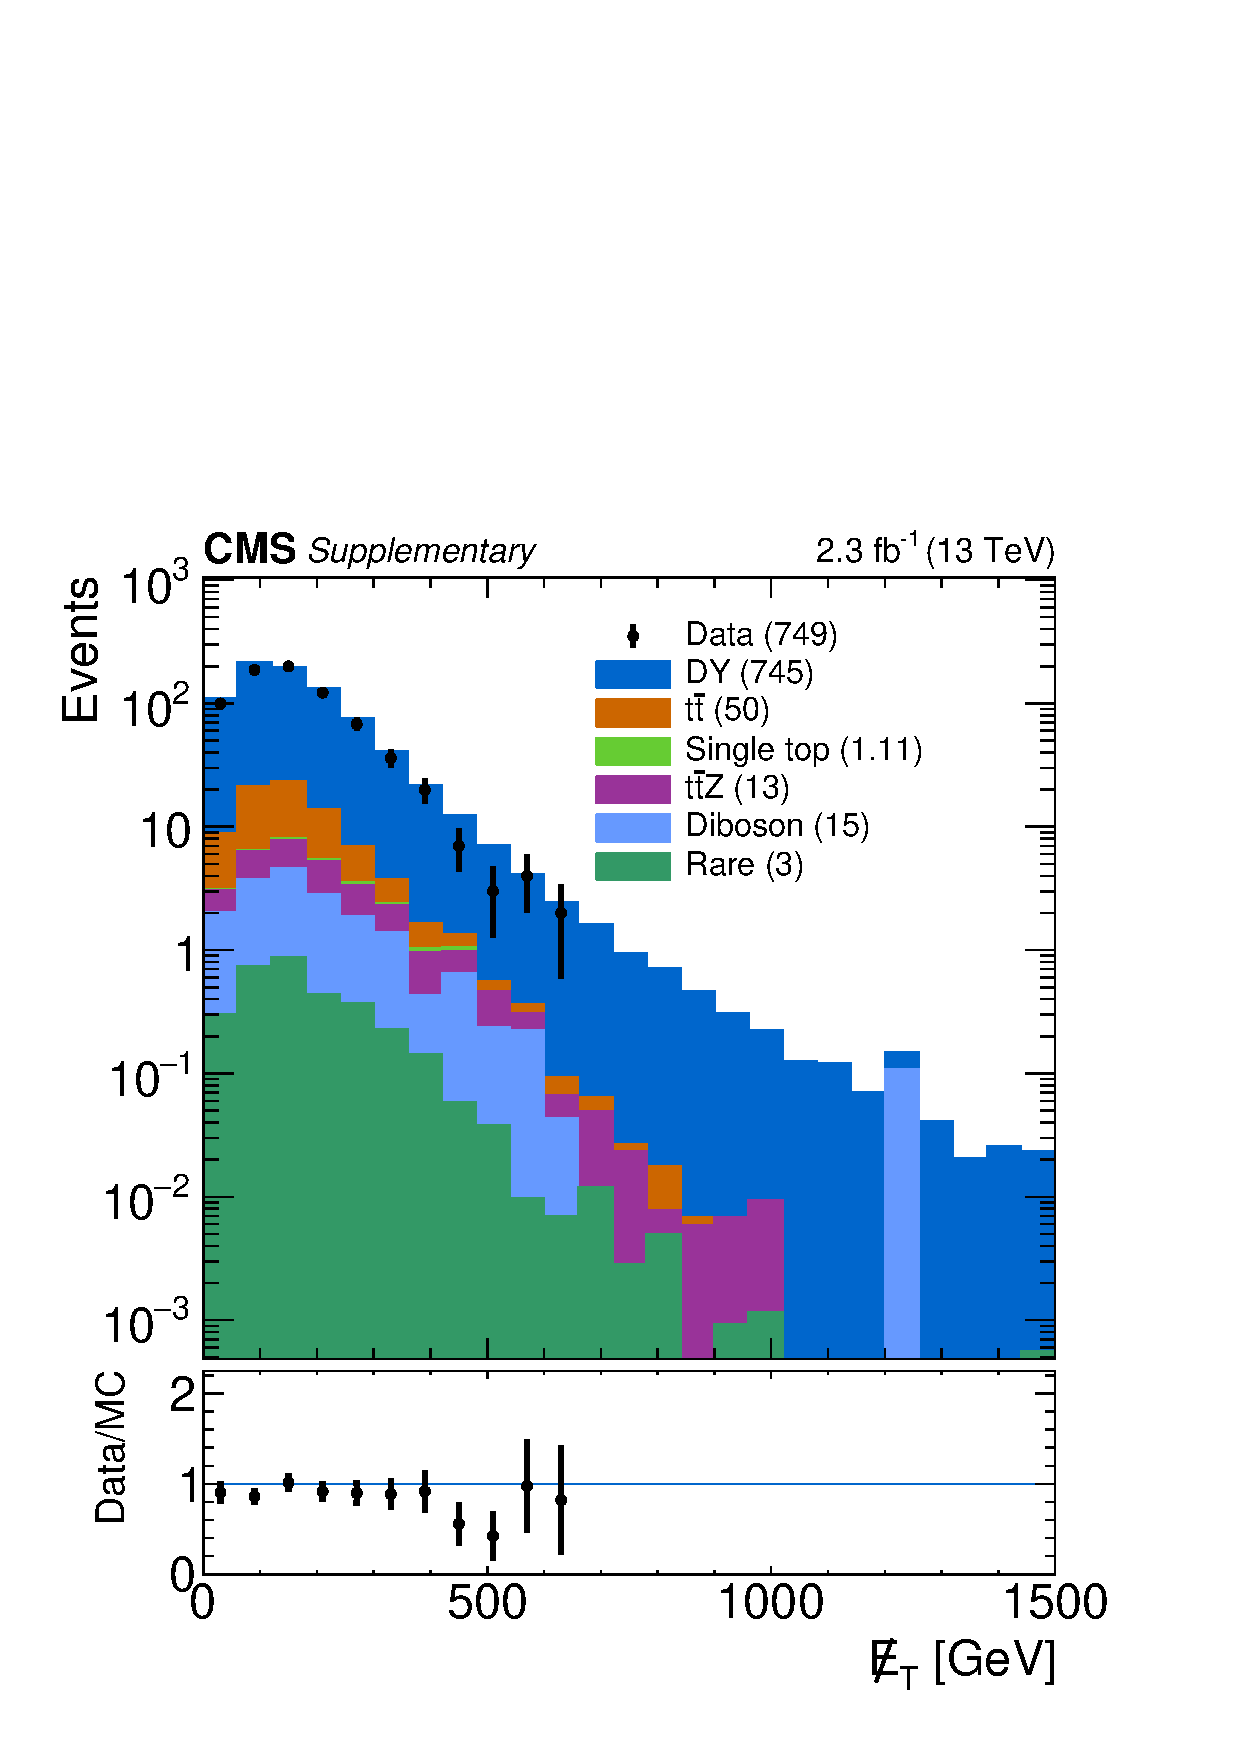
\includegraphics[width=0.5\linewidth]{figures/SusySearches/HadStop2015/DataMCw_SingleMuon_met_muZinv_loose0_ntop.pdf}
}
\subfloat[]{
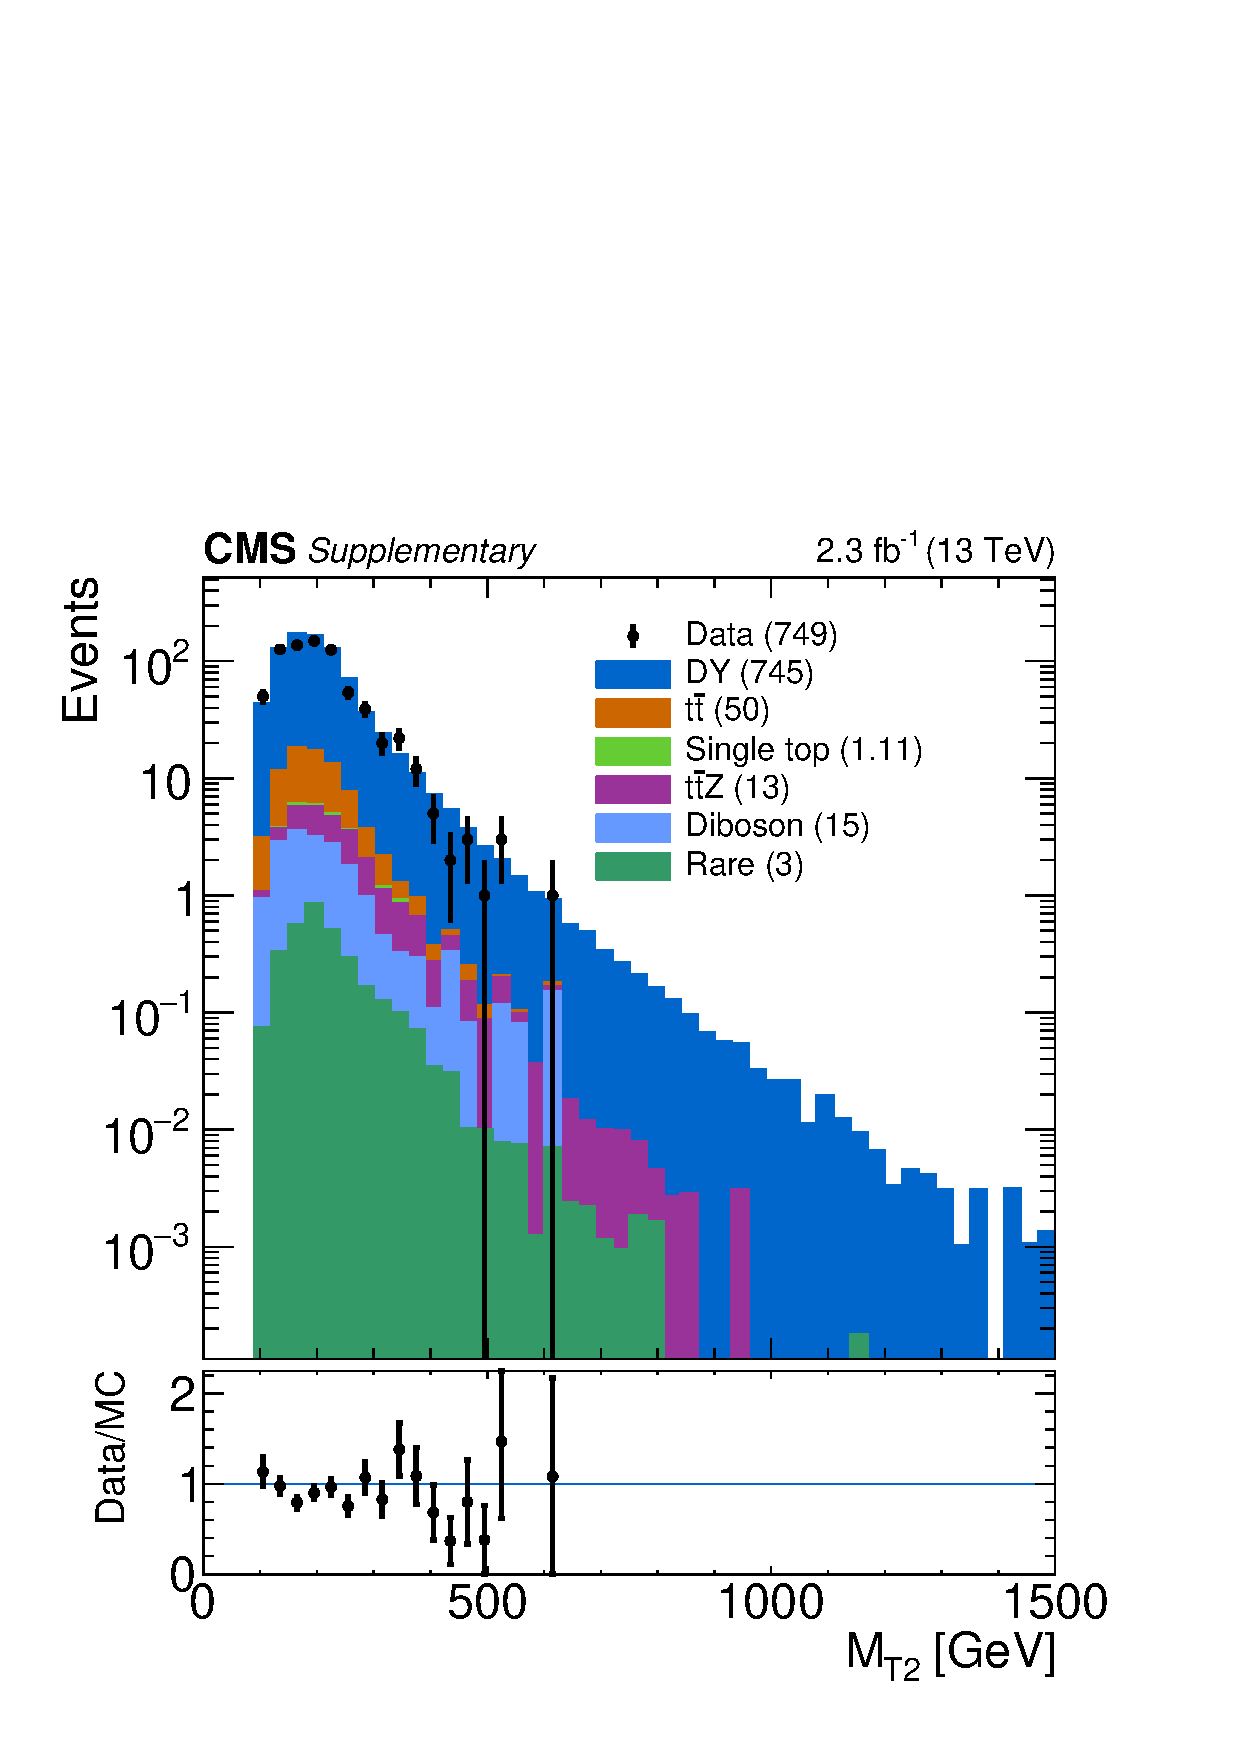
\includegraphics[width=0.5\linewidth]{figures/SusySearches/HadStop2015/DataMCw_SingleMuon_mt2_muZinv_loose0_ntop.pdf}
}\\
\subfloat[]{
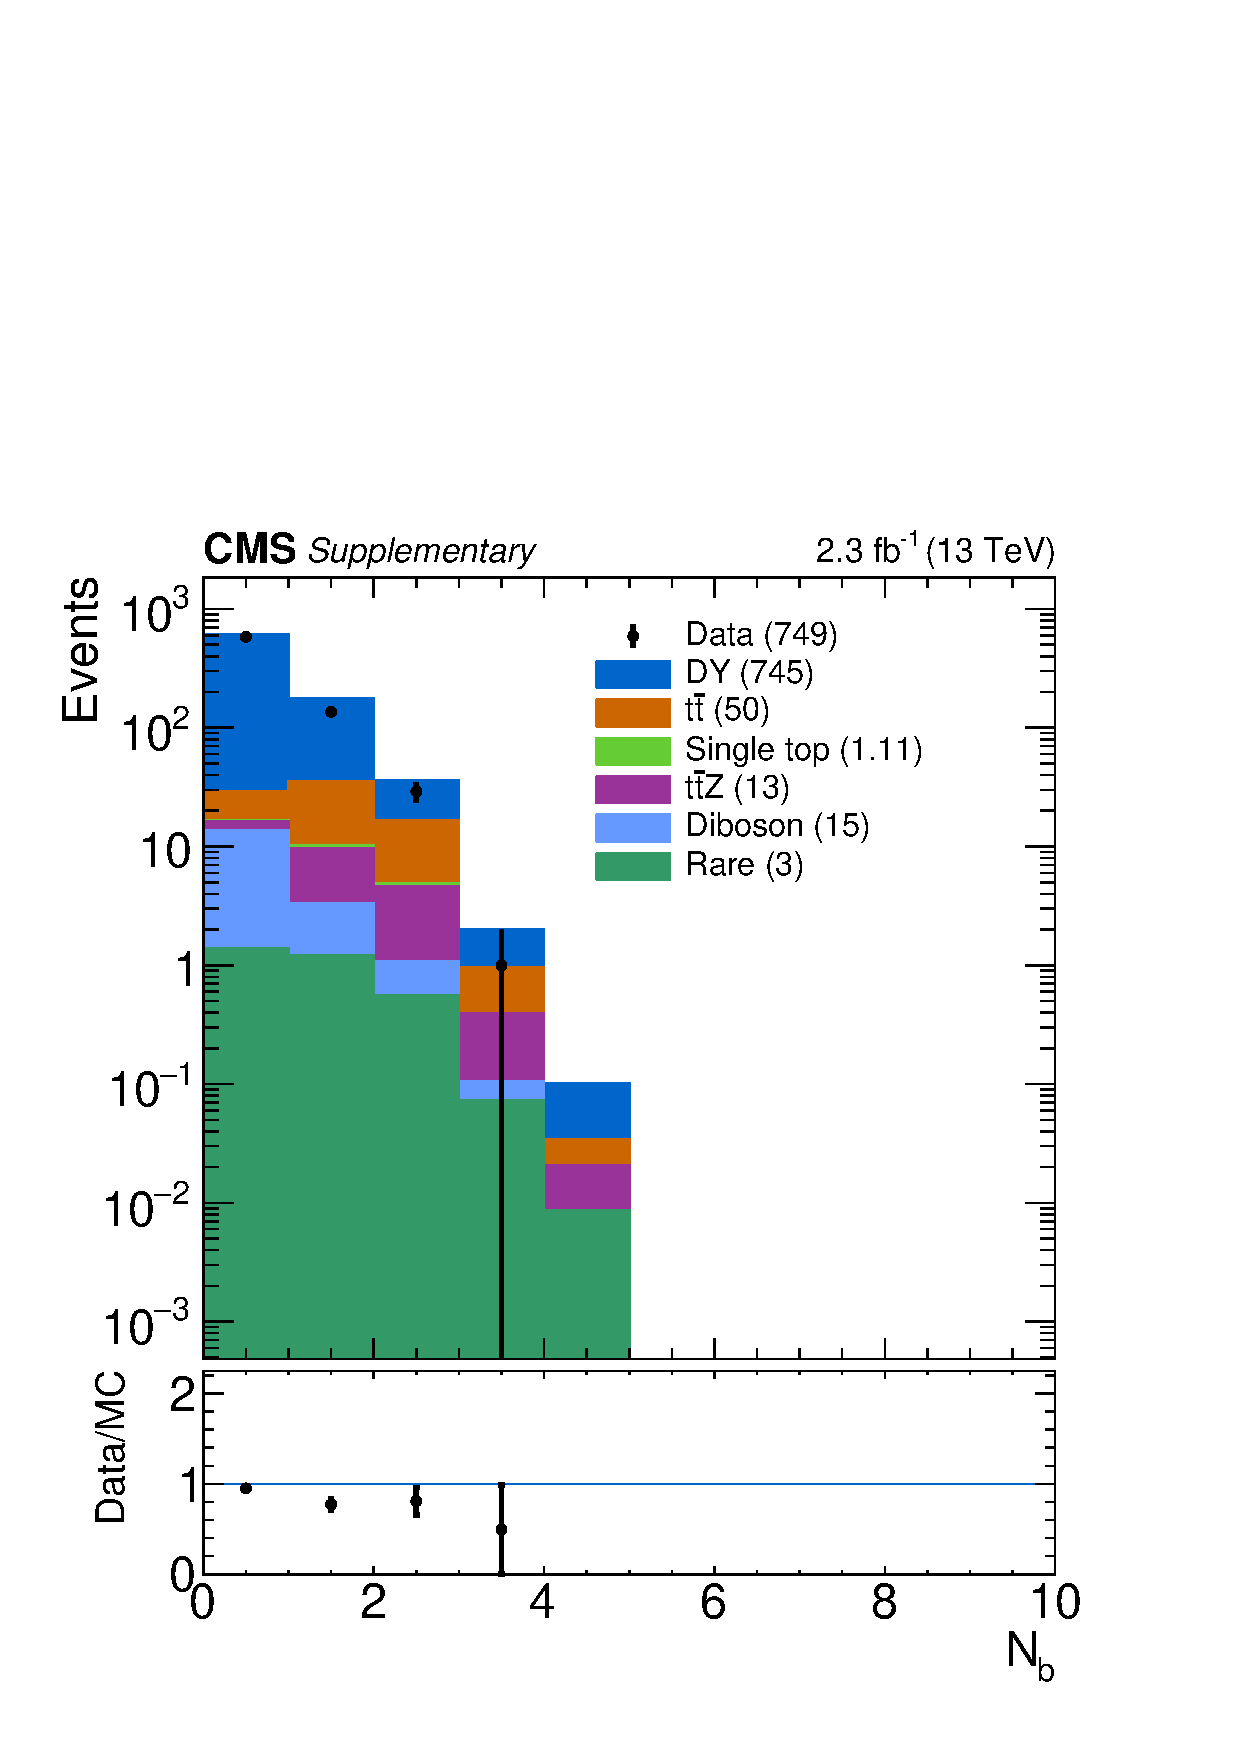
\includegraphics[width=0.5\linewidth]{figures/SusySearches/HadStop2015/DataMCw_SingleMuon_nb_muZinv_loose0_ntop.pdf}
}
\subfloat[]{
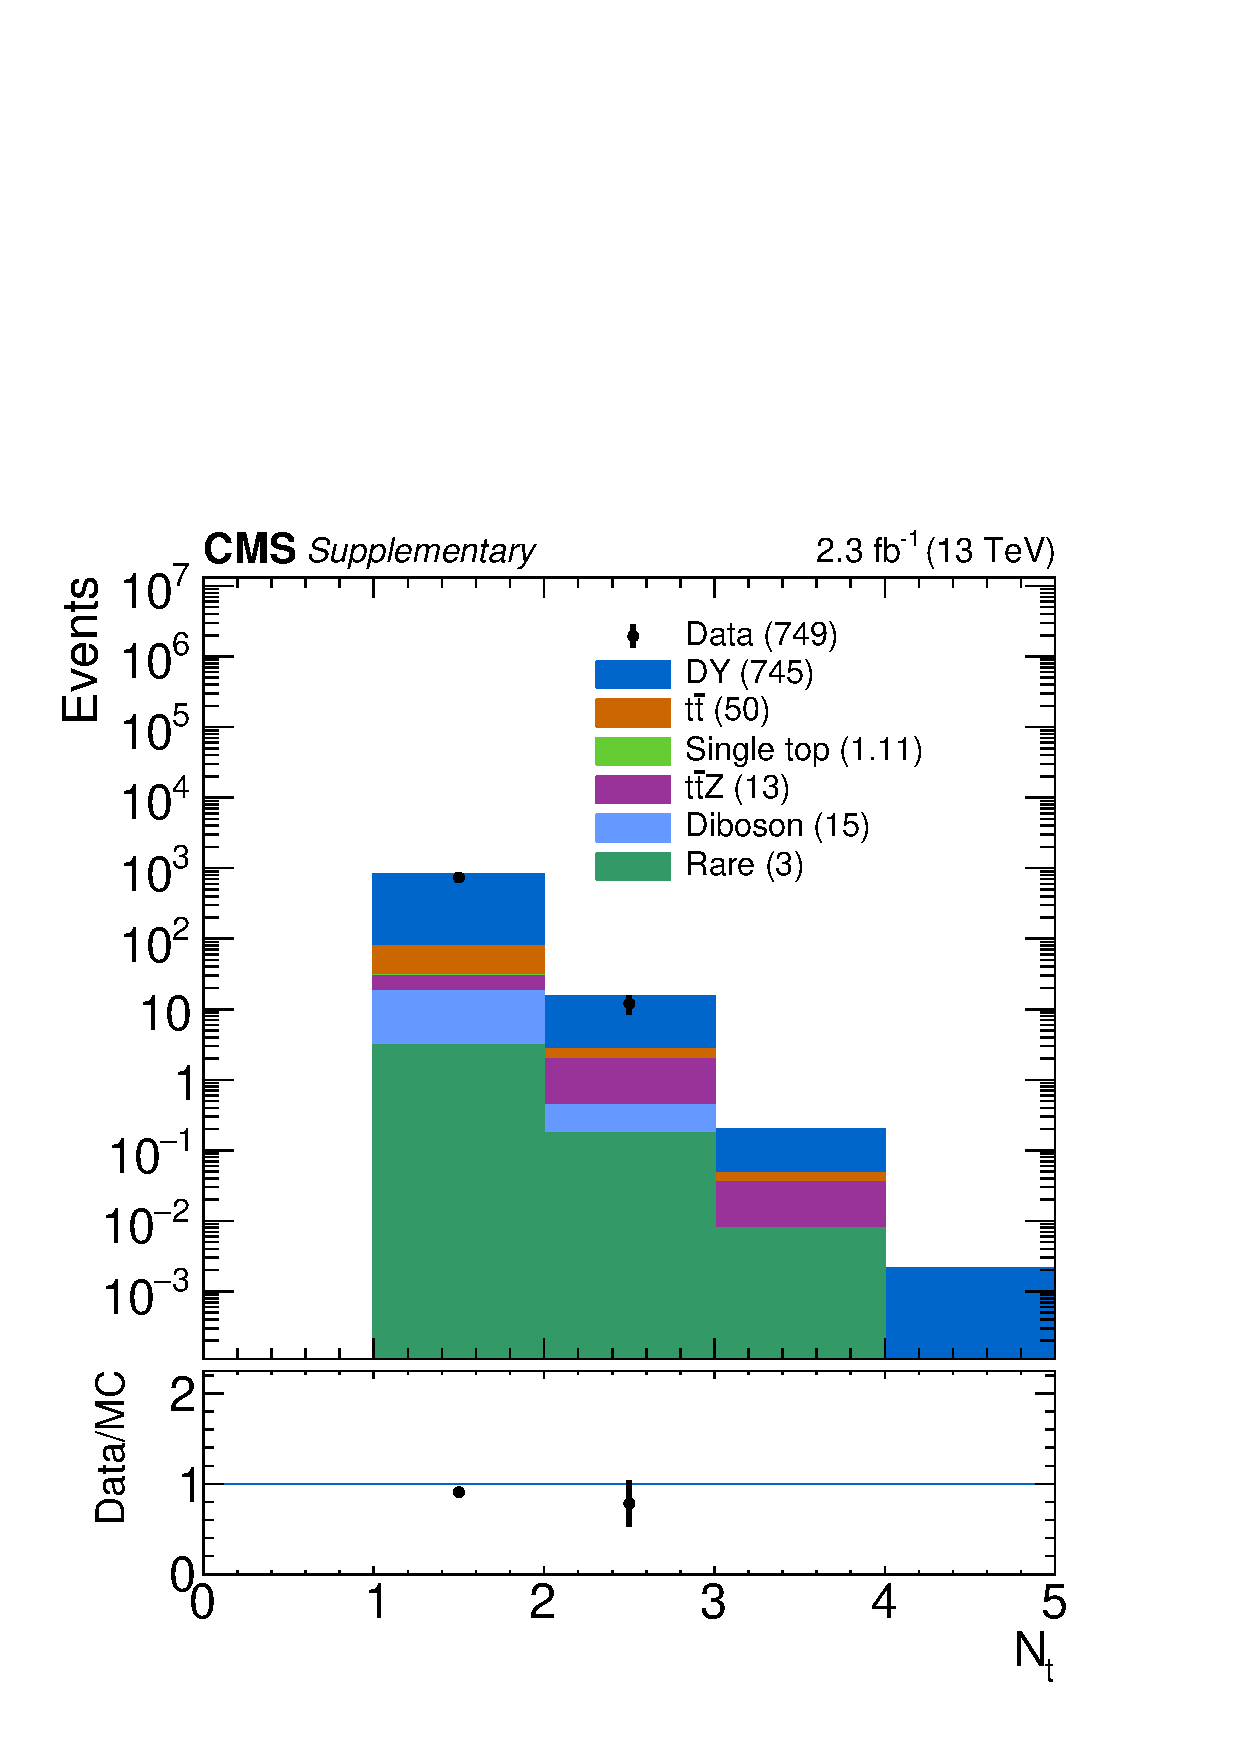
\includegraphics[width=0.5\linewidth]{figures/SusySearches/HadStop2015/DataMCw_SingleMuon_nt_muZinv_loose0_ntop.pdf}
}
\caption{Comparisons between reweighted simulation and dilepton data.}
\label{fig:zinvdatamc}
\end{figure}

The values of the uncertainties, along with the bin-by-bin prediction, for the search for SUSY in events with top-tagged jets, are given in Section \ref{sec:2015results}.

\FloatBarrier
